\documentclass[twoside]{book}

% Packages required by doxygen
\usepackage{fixltx2e}
\usepackage{calc}
\usepackage{doxygen}
\usepackage[export]{adjustbox} % also loads graphicx
\usepackage{graphicx}
\usepackage[utf8]{inputenc}
\usepackage{makeidx}
\usepackage{multicol}
\usepackage{multirow}
\PassOptionsToPackage{warn}{textcomp}
\usepackage{textcomp}
\usepackage[nointegrals]{wasysym}
\usepackage[table]{xcolor}

% Font selection
\usepackage[T1]{fontenc}
\usepackage[scaled=.90]{helvet}
\usepackage{courier}
\usepackage{amssymb}
\usepackage{sectsty}
\renewcommand{\familydefault}{\sfdefault}
\allsectionsfont{%
  \fontseries{bc}\selectfont%
  \color{darkgray}%
}
\renewcommand{\DoxyLabelFont}{%
  \fontseries{bc}\selectfont%
  \color{darkgray}%
}
\newcommand{\+}{\discretionary{\mbox{\scriptsize$\hookleftarrow$}}{}{}}

% Page & text layout
\usepackage{geometry}
\geometry{%
  a4paper,%
  top=2.5cm,%
  bottom=2.5cm,%
  left=2.5cm,%
  right=2.5cm%
}
\tolerance=750
\hfuzz=15pt
\hbadness=750
\setlength{\emergencystretch}{15pt}
\setlength{\parindent}{0cm}
\setlength{\parskip}{3ex plus 2ex minus 2ex}
\makeatletter
\renewcommand{\paragraph}{%
  \@startsection{paragraph}{4}{0ex}{-1.0ex}{1.0ex}{%
    \normalfont\normalsize\bfseries\SS@parafont%
  }%
}
\renewcommand{\subparagraph}{%
  \@startsection{subparagraph}{5}{0ex}{-1.0ex}{1.0ex}{%
    \normalfont\normalsize\bfseries\SS@subparafont%
  }%
}
\makeatother

% Headers & footers
\usepackage{fancyhdr}
\pagestyle{fancyplain}
\fancyhead[LE]{\fancyplain{}{\bfseries\thepage}}
\fancyhead[CE]{\fancyplain{}{}}
\fancyhead[RE]{\fancyplain{}{\bfseries\leftmark}}
\fancyhead[LO]{\fancyplain{}{\bfseries\rightmark}}
\fancyhead[CO]{\fancyplain{}{}}
\fancyhead[RO]{\fancyplain{}{\bfseries\thepage}}
\fancyfoot[LE]{\fancyplain{}{}}
\fancyfoot[CE]{\fancyplain{}{}}
\fancyfoot[RE]{\fancyplain{}{\bfseries\scriptsize Generated by Doxygen }}
\fancyfoot[LO]{\fancyplain{}{\bfseries\scriptsize Generated by Doxygen }}
\fancyfoot[CO]{\fancyplain{}{}}
\fancyfoot[RO]{\fancyplain{}{}}
\renewcommand{\footrulewidth}{0.4pt}
\renewcommand{\chaptermark}[1]{%
  \markboth{#1}{}%
}
\renewcommand{\sectionmark}[1]{%
  \markright{\thesection\ #1}%
}

% Indices & bibliography
\usepackage{natbib}
\usepackage[titles]{tocloft}
\setcounter{tocdepth}{3}
\setcounter{secnumdepth}{5}
\makeindex

% Hyperlinks (required, but should be loaded last)
\usepackage{ifpdf}
\ifpdf
  \usepackage[pdftex,pagebackref=true]{hyperref}
\else
  \usepackage[ps2pdf,pagebackref=true]{hyperref}
\fi
\hypersetup{%
  colorlinks=true,%
  linkcolor=blue,%
  citecolor=blue,%
  unicode%
}

% Custom commands
\newcommand{\clearemptydoublepage}{%
  \newpage{\pagestyle{empty}\cleardoublepage}%
}

\usepackage{caption}
\captionsetup{labelsep=space,justification=centering,font={bf},singlelinecheck=off,skip=4pt,position=top}

%===== C O N T E N T S =====

\begin{document}

% Titlepage & ToC
\hypersetup{pageanchor=false,
             bookmarksnumbered=true,
             pdfencoding=unicode
            }
\pagenumbering{alph}
\begin{titlepage}
\vspace*{7cm}
\begin{center}%
{\Large My Project }\\
\vspace*{1cm}
{\large Generated by Doxygen 1.8.13}\\
\end{center}
\end{titlepage}
\clearemptydoublepage
\pagenumbering{roman}
\tableofcontents
\clearemptydoublepage
\pagenumbering{arabic}
\hypersetup{pageanchor=true}

%--- Begin generated contents ---
\chapter{Namespace Index}
\section{Namespace List}
Here is a list of all namespaces with brief descriptions\+:\begin{DoxyCompactList}
\item\contentsline{section}{\hyperlink{namespaceio}{io} \\*Cet espace sera un espace permettant de définir un buffer custom pour les input, ainsi que de pouvoir afficher tout ce que l\textquotesingle{}on souhaite }{\pageref{namespaceio}}{}
\end{DoxyCompactList}

\chapter{Hierarchical Index}
\section{Class Hierarchy}
This inheritance list is sorted roughly, but not completely, alphabetically\+:\begin{DoxyCompactList}
\item \contentsline{section}{Carte}{\pageref{class_carte}}{}
\item \contentsline{section}{competence}{\pageref{classcompetence}}{}
\item \contentsline{section}{config}{\pageref{classconfig}}{}
\item \contentsline{section}{entite}{\pageref{classentite}}{}
\begin{DoxyCompactList}
\item \contentsline{section}{monstre}{\pageref{classmonstre}}{}
\item \contentsline{section}{personnage}{\pageref{classpersonnage}}{}
\end{DoxyCompactList}
\item \contentsline{section}{jeu}{\pageref{classjeu}}{}
\end{DoxyCompactList}

\chapter{Class Index}
\section{Class List}
Here are the classes, structs, unions and interfaces with brief descriptions\+:\begin{DoxyCompactList}
\item\contentsline{section}{\hyperlink{class_carte}{Carte} }{\pageref{class_carte}}{}
\item\contentsline{section}{\hyperlink{classcompetence}{competence} }{\pageref{classcompetence}}{}
\item\contentsline{section}{\hyperlink{structinterface}{interface} }{\pageref{structinterface}}{}
\item\contentsline{section}{\hyperlink{classjeu}{jeu} \\*Ceci sera la classe du jeu. Elle contient toutes les entités, la carte, ainsi que les fonctions nécessaires à la partie }{\pageref{classjeu}}{}
\item\contentsline{section}{\hyperlink{classmonstre}{monstre} }{\pageref{classmonstre}}{}
\item\contentsline{section}{\hyperlink{classpersonnage}{personnage} \\*Classe test interactions affichage }{\pageref{classpersonnage}}{}
\end{DoxyCompactList}

\chapter{File Index}
\section{File List}
Here is a list of all files with brief descriptions\+:\begin{DoxyCompactList}
\item\contentsline{section}{/\+Users/thibault/\+Git\+Hub/\+C\+E\+R\+I\+\_\+software\+\_\+engineering\+\_\+game\+\_\+1/headers/\hyperlink{carte_8h}{carte.\+h} }{\pageref{carte_8h}}{}
\item\contentsline{section}{/\+Users/thibault/\+Git\+Hub/\+C\+E\+R\+I\+\_\+software\+\_\+engineering\+\_\+game\+\_\+1/headers/\hyperlink{competence_8h}{competence.\+h} }{\pageref{competence_8h}}{}
\item\contentsline{section}{/\+Users/thibault/\+Git\+Hub/\+C\+E\+R\+I\+\_\+software\+\_\+engineering\+\_\+game\+\_\+1/headers/\hyperlink{config_8h}{config.\+h} }{\pageref{config_8h}}{}
\item\contentsline{section}{/\+Users/thibault/\+Git\+Hub/\+C\+E\+R\+I\+\_\+software\+\_\+engineering\+\_\+game\+\_\+1/headers/\hyperlink{entite_8h}{entite.\+h} }{\pageref{entite_8h}}{}
\item\contentsline{section}{/\+Users/thibault/\+Git\+Hub/\+C\+E\+R\+I\+\_\+software\+\_\+engineering\+\_\+game\+\_\+1/headers/\hyperlink{fonctionsjeu_8h}{fonctionsjeu.\+h} }{\pageref{fonctionsjeu_8h}}{}
\item\contentsline{section}{/\+Users/thibault/\+Git\+Hub/\+C\+E\+R\+I\+\_\+software\+\_\+engineering\+\_\+game\+\_\+1/headers/\hyperlink{io_8h}{io.\+h} }{\pageref{io_8h}}{}
\item\contentsline{section}{/\+Users/thibault/\+Git\+Hub/\+C\+E\+R\+I\+\_\+software\+\_\+engineering\+\_\+game\+\_\+1/headers/\hyperlink{monstre_8h}{monstre.\+h} }{\pageref{monstre_8h}}{}
\item\contentsline{section}{/\+Users/thibault/\+Git\+Hub/\+C\+E\+R\+I\+\_\+software\+\_\+engineering\+\_\+game\+\_\+1/headers/\hyperlink{personnage_8h}{personnage.\+h} }{\pageref{personnage_8h}}{}
\end{DoxyCompactList}

\chapter{Namespace Documentation}
\hypertarget{namespaceio}{}\section{io Namespace Reference}
\label{namespaceio}\index{io@{io}}


Cet espace sera un espace permettant de définir un buffer custom pour les input, ainsi que de pouvoir afficher tout ce que l\textquotesingle{}on souhaite.  


\subsection*{Functions}
\begin{DoxyCompactItemize}
\item 
\mbox{\Hypertarget{namespaceio_aa3dbf94851f627ae6201efa77e77198c}\label{namespaceio_aa3dbf94851f627ae6201efa77e77198c}} 
std\+::istream {\bfseries io\+\_\+input} ()
\item 
char \hyperlink{namespaceio_ae9908b55f26f07e78043d7cfad003d22}{de} ()
\begin{DoxyCompactList}\small\item\em Input. \end{DoxyCompactList}\item 
void \hyperlink{namespaceio_a7fdf85a0d766d2dcdb9870ae0458826a}{bienvenue} ()
\begin{DoxyCompactList}\small\item\em Message d\textquotesingle{}accueil. \end{DoxyCompactList}\item 
\mbox{\Hypertarget{namespaceio_a71636a15a219ee1dcc177e9749cf20bc}\label{namespaceio_a71636a15a219ee1dcc177e9749cf20bc}} 
int \hyperlink{namespaceio_a71636a15a219ee1dcc177e9749cf20bc}{get\+Terminal\+Width} ()
\begin{DoxyCompactList}\small\item\em Retourne la largeur du terminal. \end{DoxyCompactList}\item 
\mbox{\Hypertarget{namespaceio_ab7da8a98a7b636d1d5f0f6eb820f1f81}\label{namespaceio_ab7da8a98a7b636d1d5f0f6eb820f1f81}} 
int \hyperlink{namespaceio_ab7da8a98a7b636d1d5f0f6eb820f1f81}{get\+Terminal\+Height} ()
\begin{DoxyCompactList}\small\item\em Retourne la hauteur du terminal. \end{DoxyCompactList}\item 
{\footnotesize template$<$typename T $>$ }\\void \hyperlink{namespaceio_a0e3593d732c42572e8b3cb09ad21c4c9}{afficher} (T object, bool need\+\_\+desc)
\begin{DoxyCompactList}\small\item\em Affichage d\textquotesingle{}objet. \end{DoxyCompactList}\item 
{\footnotesize template$<$typename T $>$ }\\void \hyperlink{namespaceio_a0518bc32f1debefc2630431cd0c22cb0}{liste\+\_\+elements} (std\+::vector$<$ T $>$ vect\+\_\+element, bool need\+\_\+desc)
\begin{DoxyCompactList}\small\item\em Affichage d\textquotesingle{}un ensemble d\textquotesingle{}objets. \end{DoxyCompactList}\item 
{\footnotesize template$<$typename T $>$ }\\T \hyperlink{namespaceio_af398625b832f98bc758b9ea7665a168e}{choix\+\_\+unique\+\_\+element} (std\+::vector$<$ T $>$ vect\+\_\+element, bool need\+\_\+desc)
\begin{DoxyCompactList}\small\item\em Choix d\textquotesingle{}un élément unique. \end{DoxyCompactList}\end{DoxyCompactItemize}


\subsection{Detailed Description}
Cet espace sera un espace permettant de définir un buffer custom pour les input, ainsi que de pouvoir afficher tout ce que l\textquotesingle{}on souhaite. 

\subsection{Function Documentation}
\mbox{\Hypertarget{namespaceio_a0e3593d732c42572e8b3cb09ad21c4c9}\label{namespaceio_a0e3593d732c42572e8b3cb09ad21c4c9}} 
\index{io@{io}!afficher@{afficher}}
\index{afficher@{afficher}!io@{io}}
\subsubsection{\texorpdfstring{afficher()}{afficher()}}
{\footnotesize\ttfamily template$<$typename T $>$ \\
void io\+::afficher (\begin{DoxyParamCaption}\item[{T}]{object,  }\item[{bool}]{need\+\_\+desc }\end{DoxyParamCaption})}



Affichage d\textquotesingle{}objet. 

Affiche le nom (et éventuellement la description) d\textquotesingle{}un objet. 
\begin{DoxyParams}{Parameters}
{\em object} & Objet à afficher. \\
\hline
{\em need\+\_\+desc} & Description ou non. \\
\hline
\end{DoxyParams}
\mbox{\Hypertarget{namespaceio_a7fdf85a0d766d2dcdb9870ae0458826a}\label{namespaceio_a7fdf85a0d766d2dcdb9870ae0458826a}} 
\index{io@{io}!bienvenue@{bienvenue}}
\index{bienvenue@{bienvenue}!io@{io}}
\subsubsection{\texorpdfstring{bienvenue()}{bienvenue()}}
{\footnotesize\ttfamily void io\+::bienvenue (\begin{DoxyParamCaption}{ }\end{DoxyParamCaption})}



Message d\textquotesingle{}accueil. 

Affiche un message de bienvenue. \mbox{\Hypertarget{namespaceio_af398625b832f98bc758b9ea7665a168e}\label{namespaceio_af398625b832f98bc758b9ea7665a168e}} 
\index{io@{io}!choix\+\_\+unique\+\_\+element@{choix\+\_\+unique\+\_\+element}}
\index{choix\+\_\+unique\+\_\+element@{choix\+\_\+unique\+\_\+element}!io@{io}}
\subsubsection{\texorpdfstring{choix\+\_\+unique\+\_\+element()}{choix\_unique\_element()}}
{\footnotesize\ttfamily template$<$typename T $>$ \\
T io\+::choix\+\_\+unique\+\_\+element (\begin{DoxyParamCaption}\item[{std\+::vector$<$ T $>$}]{vect\+\_\+element,  }\item[{bool}]{need\+\_\+desc }\end{DoxyParamCaption})}



Choix d\textquotesingle{}un élément unique. 

Fonction qui prend un vecteur d\textquotesingle{}éléments en entrée ainsi qu\textquotesingle{}un booléen (affichage ou non de la description), et affiche puis renvoie l\textquotesingle{}élément choisi. 
\begin{DoxyParams}{Parameters}
{\em vect\+\_\+element} & Vecteur de l\textquotesingle{}élément à choisir. \\
\hline
{\em need\+\_\+desc} & Nécessité de description ou non. \\
\hline
\end{DoxyParams}
\begin{DoxyReturn}{Returns}
L\textquotesingle{}élement choisi. 
\end{DoxyReturn}
\begin{DoxySeeAlso}{See also}
\hyperlink{namespaceio_a0518bc32f1debefc2630431cd0c22cb0}{liste\+\_\+elements()}, \hyperlink{namespaceio_a0e3593d732c42572e8b3cb09ad21c4c9}{afficher()} 
\end{DoxySeeAlso}
\mbox{\Hypertarget{namespaceio_ae9908b55f26f07e78043d7cfad003d22}\label{namespaceio_ae9908b55f26f07e78043d7cfad003d22}} 
\index{io@{io}!de@{de}}
\index{de@{de}!io@{io}}
\subsubsection{\texorpdfstring{de()}{de()}}
{\footnotesize\ttfamily char io\+::de (\begin{DoxyParamCaption}{ }\end{DoxyParamCaption})}



Input. 

Gestion des entrées utilisateur. \mbox{\Hypertarget{namespaceio_a0518bc32f1debefc2630431cd0c22cb0}\label{namespaceio_a0518bc32f1debefc2630431cd0c22cb0}} 
\index{io@{io}!liste\+\_\+elements@{liste\+\_\+elements}}
\index{liste\+\_\+elements@{liste\+\_\+elements}!io@{io}}
\subsubsection{\texorpdfstring{liste\+\_\+elements()}{liste\_elements()}}
{\footnotesize\ttfamily template$<$typename T $>$ \\
void io\+::liste\+\_\+elements (\begin{DoxyParamCaption}\item[{std\+::vector$<$ T $>$}]{vect\+\_\+element,  }\item[{bool}]{need\+\_\+desc }\end{DoxyParamCaption})}



Affichage d\textquotesingle{}un ensemble d\textquotesingle{}objets. 

Parcourt le vecteur de stockage des objets chargés, et les affiche. 
\begin{DoxyParams}{Parameters}
{\em vect\+\_\+element} & Vecteur d\textquotesingle{}éléments. \\
\hline
{\em need\+\_\+desc} & Description ou non. \\
\hline
\end{DoxyParams}
\begin{DoxySeeAlso}{See also}
\hyperlink{namespaceio_a0e3593d732c42572e8b3cb09ad21c4c9}{afficher()} 
\end{DoxySeeAlso}

\chapter{Class Documentation}
\hypertarget{class_carte}{}\section{Carte Class Reference}
\label{class_carte}\index{Carte@{Carte}}
\subsection*{Public Member Functions}
\begin{DoxyCompactItemize}
\item 
\mbox{\Hypertarget{class_carte_a23c6f00e5cc97f469b8f8de4e37f54a9}\label{class_carte_a23c6f00e5cc97f469b8f8de4e37f54a9}} 
{\bfseries Carte} (int taille, std\+::string name, std\+::string description)
\item 
\mbox{\Hypertarget{class_carte_aed4a23fad7ef43f46f80dbff08468cc9}\label{class_carte_aed4a23fad7ef43f46f80dbff08468cc9}} 
void {\bfseries affichage} ()
\item 
\mbox{\Hypertarget{class_carte_aceb1051f87ed3c407bfcf25fe4cc7778}\label{class_carte_aceb1051f87ed3c407bfcf25fe4cc7778}} 
void {\bfseries sauvegarde} ()
\item 
\mbox{\Hypertarget{class_carte_a376e889c21215615bfa3b5068f46e646}\label{class_carte_a376e889c21215615bfa3b5068f46e646}} 
std\+::string {\bfseries get\+Name} ()
\item 
\mbox{\Hypertarget{class_carte_a591705d6bb95c36ce4a034b3107ae85c}\label{class_carte_a591705d6bb95c36ce4a034b3107ae85c}} 
std\+::string {\bfseries get\+Description} ()
\item 
\mbox{\Hypertarget{class_carte_a25815ab5ece47d7df6fa5b845d03c785}\label{class_carte_a25815ab5ece47d7df6fa5b845d03c785}} 
bool {\bfseries carte\+\_\+existe} (std\+::string nom)
\item 
\mbox{\Hypertarget{class_carte_a3c64f88c1798cd90997f9835d06c81cc}\label{class_carte_a3c64f88c1798cd90997f9835d06c81cc}} 
void {\bfseries chargement} (std\+::string nom\+\_\+selection)
\item 
\mbox{\Hypertarget{class_carte_a0aa64d23c01e359285a557c847d71828}\label{class_carte_a0aa64d23c01e359285a557c847d71828}} 
int {\bfseries quel\+\_\+taille} (std\+::string nom)
\item 
\mbox{\Hypertarget{class_carte_a5e06941d4f9af38e63b187f61277ba4d}\label{class_carte_a5e06941d4f9af38e63b187f61277ba4d}} 
void {\bfseries suppression} (std\+::string nom)
\end{DoxyCompactItemize}


The documentation for this class was generated from the following file\+:\begin{DoxyCompactItemize}
\item 
/\+Users/thibault/\+Git\+Hub/\+C\+E\+R\+I\+\_\+software\+\_\+engineering\+\_\+game\+\_\+1/headers/carte.\+h\end{DoxyCompactItemize}

\hypertarget{classcompetence}{}\section{competence Class Reference}
\label{classcompetence}\index{competence@{competence}}


{\ttfamily \#include $<$competence.\+h$>$}

\subsection*{Public Member Functions}
\begin{DoxyCompactItemize}
\item 
\hyperlink{classcompetence_ae47bad4331015d873fef6b006b987d38}{competence} ()
\begin{DoxyCompactList}\small\item\em Constructeur sans arguments. \end{DoxyCompactList}\item 
\hyperlink{classcompetence_ae214635d91c8b1c5a37352dccbcd2397}{competence} (std\+::string skill\+Name, int skill\+Damage, int skill\+Mana\+Cost)
\begin{DoxyCompactList}\small\item\em Constructeur permettant de créer une compétence pour un personnage. \end{DoxyCompactList}\item 
\hyperlink{classcompetence_a269947808c5e8662ecabb11e96a4d9c0}{competence} (std\+::string skill\+Name, int skill\+Damage)
\begin{DoxyCompactList}\small\item\em Constructeur permettant de créer une compétence pour un monstre. \end{DoxyCompactList}\item 
\hyperlink{classcompetence_a158b19a476ae306eeaaa6672aab62e6c}{$\sim$competence} ()
\begin{DoxyCompactList}\small\item\em Destructeur de compétence. \end{DoxyCompactList}\item 
std\+::string \hyperlink{classcompetence_abbb996751e239fc151caae2a73947710}{get\+Name} ()
\begin{DoxyCompactList}\small\item\em Fonction retournant le nom d\textquotesingle{}une compétence. \end{DoxyCompactList}\item 
std\+::string \hyperlink{classcompetence_ae0980a623fb74c32a630400cdb56cd14}{get\+Description} ()
\begin{DoxyCompactList}\small\item\em Fonction retournant la description d\textquotesingle{}une compétence. \end{DoxyCompactList}\item 
int \hyperlink{classcompetence_a752380fae93494815023b3a177e57f44}{get\+Damage} ()
\begin{DoxyCompactList}\small\item\em Fonction retournant le nombre de points de dégâts à appliquer à une cible. \end{DoxyCompactList}\item 
int \hyperlink{classcompetence_a8346c6ae95df148e42f26b9a94655c8f}{get\+Mana\+Cost} ()
\begin{DoxyCompactList}\small\item\em Fonction retournant le nombre de points de magie à utiliser. \end{DoxyCompactList}\item 
{\footnotesize template$<$typename T $>$ }\\std\+::string \hyperlink{classcompetence_adbd67d184b75c46bc22c1aef070d9246}{to\+String} (const T \&valeur)
\begin{DoxyCompactList}\small\item\em Template permettant de retourner une string contenant un élément. \end{DoxyCompactList}\item 
void \hyperlink{classcompetence_a8398d16c43f6ca6b44e3779730e022b6}{afficher\+\_\+detail} ()
\begin{DoxyCompactList}\small\item\em Affichage d\textquotesingle{}une compétence. \end{DoxyCompactList}\item 
std\+::string \hyperlink{classcompetence_a7e0e1108a22437875609defae6515f09}{afficher\+\_\+detail\+\_\+combat} ()
\item 
std\+::string \hyperlink{classcompetence_a4acc4e02f7e8c49a6d4d1db307e8f03d}{competence\+String} ()
\begin{DoxyCompactList}\small\item\em Conversion en string. \end{DoxyCompactList}\end{DoxyCompactItemize}


\subsection{Detailed Description}
Permet de contenir une compétence en mémoire.

Une compétence est formée grâce à \+:
\begin{DoxyItemize}
\item un nom ({\ttfamily skill\+Name})
\item un nombre de points de dégâts à appliquer (si ce nombre est négatif, la compétence permet de soigner une cible)
\item un coût en points de magie (si ce nombre est négatif, la compétence permet de régénerer des points de magie)
\end{DoxyItemize}

N\+O\+TE \+: Par convention, une compétence qui contient un nombre de points de mana sera utilisée sur un joueur. Un monstre n\textquotesingle{}a pas de magie à gérer. 

\subsection{Constructor \& Destructor Documentation}
\mbox{\Hypertarget{classcompetence_ae47bad4331015d873fef6b006b987d38}\label{classcompetence_ae47bad4331015d873fef6b006b987d38}} 
\index{competence@{competence}!competence@{competence}}
\index{competence@{competence}!competence@{competence}}
\subsubsection{\texorpdfstring{competence()}{competence()}\hspace{0.1cm}{\footnotesize\ttfamily [1/3]}}
{\footnotesize\ttfamily competence\+::competence (\begin{DoxyParamCaption}{ }\end{DoxyParamCaption})}



Constructeur sans arguments. 

En sortant de ce constructeur, la compétence aura \+:
\begin{DoxyItemize}
\item skill\+Name = \char`\"{}\+Inconnu\char`\"{}
\item skill\+Damage = 0
\item skill\+Mana\+Cost = 0 
\end{DoxyItemize}\mbox{\Hypertarget{classcompetence_ae214635d91c8b1c5a37352dccbcd2397}\label{classcompetence_ae214635d91c8b1c5a37352dccbcd2397}} 
\index{competence@{competence}!competence@{competence}}
\index{competence@{competence}!competence@{competence}}
\subsubsection{\texorpdfstring{competence()}{competence()}\hspace{0.1cm}{\footnotesize\ttfamily [2/3]}}
{\footnotesize\ttfamily competence\+::competence (\begin{DoxyParamCaption}\item[{std\+::string}]{skill\+Name,  }\item[{int}]{skill\+Damage,  }\item[{int}]{skill\+Mana\+Cost }\end{DoxyParamCaption})}



Constructeur permettant de créer une compétence pour un personnage. 

Les compétences créées avec ce constructeur seront utilisées pour un personnage. La compétence aura donc comme données \+:
\begin{DoxyItemize}
\item competence\+::skill\+Name = skill\+Name
\item competence\+::skill\+Damage = skill\+Damage
\item competence\+::skill\+Mana\+Cost = skill\+Mana\+Cost 
\begin{DoxyParams}{Parameters}
{\em skill\+Name} & Nom à assigner à la compétence \\
\hline
{\em skill\+Damage} & Nombre de points de vie à assigner à la compétence (si ce nombre est négatif, la compétence permet de soigner une cible) \\
\hline
{\em skill\+Mana\+Cost} & Nombre de points de magie à assigner à la compétence (si ce nombre est négatif, la compétence permet de régénerer des points de magie) \\
\hline
\end{DoxyParams}

\end{DoxyItemize}\mbox{\Hypertarget{classcompetence_a269947808c5e8662ecabb11e96a4d9c0}\label{classcompetence_a269947808c5e8662ecabb11e96a4d9c0}} 
\index{competence@{competence}!competence@{competence}}
\index{competence@{competence}!competence@{competence}}
\subsubsection{\texorpdfstring{competence()}{competence()}\hspace{0.1cm}{\footnotesize\ttfamily [3/3]}}
{\footnotesize\ttfamily competence\+::competence (\begin{DoxyParamCaption}\item[{std\+::string}]{skill\+Name,  }\item[{int}]{skill\+Damage }\end{DoxyParamCaption})}



Constructeur permettant de créer une compétence pour un monstre. 

Les compétences créées avec ce constructeur seront utilisées pour un monstre. La compétence aura donc comme données \+:
\begin{DoxyItemize}
\item competence\+::skill\+Name = skill\+Name
\item competence\+::skill\+Damage = skill\+Damage 
\begin{DoxyParams}{Parameters}
{\em skill\+Name} & Nom à assigner à la compétence \\
\hline
{\em skill\+Damage} & Nombre de points de vie à assigner à la compétence (si ce nombre est négatif, la compétence permet de soigner une cible) \\
\hline
\end{DoxyParams}
\begin{DoxyNote}{Note}
Les compétences créées utilisant ce constructeur seront assignées à des monstres. Par convention, un monstre n\textquotesingle{}a pas à gérer de magie. 
\end{DoxyNote}

\end{DoxyItemize}\mbox{\Hypertarget{classcompetence_a158b19a476ae306eeaaa6672aab62e6c}\label{classcompetence_a158b19a476ae306eeaaa6672aab62e6c}} 
\index{competence@{competence}!````~competence@{$\sim$competence}}
\index{````~competence@{$\sim$competence}!competence@{competence}}
\subsubsection{\texorpdfstring{$\sim$competence()}{~competence()}}
{\footnotesize\ttfamily competence\+::$\sim$competence (\begin{DoxyParamCaption}{ }\end{DoxyParamCaption})}



Destructeur de compétence. 



\subsection{Member Function Documentation}
\mbox{\Hypertarget{classcompetence_a8398d16c43f6ca6b44e3779730e022b6}\label{classcompetence_a8398d16c43f6ca6b44e3779730e022b6}} 
\index{competence@{competence}!afficher\+\_\+detail@{afficher\+\_\+detail}}
\index{afficher\+\_\+detail@{afficher\+\_\+detail}!competence@{competence}}
\subsubsection{\texorpdfstring{afficher\+\_\+detail()}{afficher\_detail()}}
{\footnotesize\ttfamily void competence\+::afficher\+\_\+detail (\begin{DoxyParamCaption}{ }\end{DoxyParamCaption})}



Affichage d\textquotesingle{}une compétence. 

Affiche les éléments détaillés d\textquotesingle{}une compétence (nom, dégâts, coût). Si les dégâts sont négatifs, affiche \char`\"{}soins\char`\"{}. Si le coût est négatif, affiche \char`\"{}gain\char`\"{}. \mbox{\Hypertarget{classcompetence_a7e0e1108a22437875609defae6515f09}\label{classcompetence_a7e0e1108a22437875609defae6515f09}} 
\index{competence@{competence}!afficher\+\_\+detail\+\_\+combat@{afficher\+\_\+detail\+\_\+combat}}
\index{afficher\+\_\+detail\+\_\+combat@{afficher\+\_\+detail\+\_\+combat}!competence@{competence}}
\subsubsection{\texorpdfstring{afficher\+\_\+detail\+\_\+combat()}{afficher\_detail\_combat()}}
{\footnotesize\ttfamily std\+::string competence\+::afficher\+\_\+detail\+\_\+combat (\begin{DoxyParamCaption}{ }\end{DoxyParamCaption})}

\mbox{\Hypertarget{classcompetence_a4acc4e02f7e8c49a6d4d1db307e8f03d}\label{classcompetence_a4acc4e02f7e8c49a6d4d1db307e8f03d}} 
\index{competence@{competence}!competence\+String@{competence\+String}}
\index{competence\+String@{competence\+String}!competence@{competence}}
\subsubsection{\texorpdfstring{competence\+String()}{competenceString()}}
{\footnotesize\ttfamily std\+::string competence\+::competence\+String (\begin{DoxyParamCaption}{ }\end{DoxyParamCaption})}



Conversion en string. 

Permet de convertir les caractéristiques d\textquotesingle{}une compétence en chaîne de caractère en vue de son écriture dans un fichier \begin{DoxyReturn}{Returns}
Un string correspondant à la compétence 
\end{DoxyReturn}
\mbox{\Hypertarget{classcompetence_a752380fae93494815023b3a177e57f44}\label{classcompetence_a752380fae93494815023b3a177e57f44}} 
\index{competence@{competence}!get\+Damage@{get\+Damage}}
\index{get\+Damage@{get\+Damage}!competence@{competence}}
\subsubsection{\texorpdfstring{get\+Damage()}{getDamage()}}
{\footnotesize\ttfamily int competence\+::get\+Damage (\begin{DoxyParamCaption}{ }\end{DoxyParamCaption})}



Fonction retournant le nombre de points de dégâts à appliquer à une cible. 

Est utilisée notemment pour l\textquotesingle{}affichage des possibilités du joueur pendant le combat contre un (des) \hyperlink{classmonstre}{monstre(s)}. \begin{DoxyReturn}{Returns}
Un entier ({\ttfamily int}) contenant le nombre de points de dégâts à appliquer à une cible. 
\end{DoxyReturn}
\mbox{\Hypertarget{classcompetence_ae0980a623fb74c32a630400cdb56cd14}\label{classcompetence_ae0980a623fb74c32a630400cdb56cd14}} 
\index{competence@{competence}!get\+Description@{get\+Description}}
\index{get\+Description@{get\+Description}!competence@{competence}}
\subsubsection{\texorpdfstring{get\+Description()}{getDescription()}}
{\footnotesize\ttfamily std\+::string competence\+::get\+Description (\begin{DoxyParamCaption}{ }\end{DoxyParamCaption})}



Fonction retournant la description d\textquotesingle{}une compétence. 

Est utilisée notemment pour l\textquotesingle{}affichage des possibilités du joueur pendant le combat contre un (des) \hyperlink{classmonstre}{monstre(s)}. \begin{DoxyReturn}{Returns}
Une string ({\ttfamily std\+::string}) contenant la description. 
\end{DoxyReturn}
\mbox{\Hypertarget{classcompetence_a8346c6ae95df148e42f26b9a94655c8f}\label{classcompetence_a8346c6ae95df148e42f26b9a94655c8f}} 
\index{competence@{competence}!get\+Mana\+Cost@{get\+Mana\+Cost}}
\index{get\+Mana\+Cost@{get\+Mana\+Cost}!competence@{competence}}
\subsubsection{\texorpdfstring{get\+Mana\+Cost()}{getManaCost()}}
{\footnotesize\ttfamily int competence\+::get\+Mana\+Cost (\begin{DoxyParamCaption}{ }\end{DoxyParamCaption})}



Fonction retournant le nombre de points de magie à utiliser. 

Est utilisée notemment pour l\textquotesingle{}affichage des possibilités du joueur pendant le combat contre un (des) \hyperlink{classmonstre}{monstre(s)}. \begin{DoxyReturn}{Returns}
Un entier ({\ttfamily int}) contenant le nombre de points de magie à utiliser. 
\end{DoxyReturn}
\mbox{\Hypertarget{classcompetence_abbb996751e239fc151caae2a73947710}\label{classcompetence_abbb996751e239fc151caae2a73947710}} 
\index{competence@{competence}!get\+Name@{get\+Name}}
\index{get\+Name@{get\+Name}!competence@{competence}}
\subsubsection{\texorpdfstring{get\+Name()}{getName()}}
{\footnotesize\ttfamily std\+::string competence\+::get\+Name (\begin{DoxyParamCaption}{ }\end{DoxyParamCaption})}



Fonction retournant le nom d\textquotesingle{}une compétence. 

Est utilisée notemment pour l\textquotesingle{}affichage des possibilités du joueur pendant le combat contre un (des) \hyperlink{classmonstre}{monstre(s)}. \begin{DoxyReturn}{Returns}
Une string ({\ttfamily std\+::string}) contenant le nom. 
\end{DoxyReturn}
\mbox{\Hypertarget{classcompetence_adbd67d184b75c46bc22c1aef070d9246}\label{classcompetence_adbd67d184b75c46bc22c1aef070d9246}} 
\index{competence@{competence}!to\+String@{to\+String}}
\index{to\+String@{to\+String}!competence@{competence}}
\subsubsection{\texorpdfstring{to\+String()}{toString()}}
{\footnotesize\ttfamily template$<$typename T $>$ \\
std\+::string competence\+::to\+String (\begin{DoxyParamCaption}\item[{const T \&}]{valeur }\end{DoxyParamCaption})}



Template permettant de retourner une string contenant un élément. 

Template permettant de retourner une string ({\ttfamily std\+::string}) contenant un élément de la classe {\ttfamily T} en forme de string. \begin{DoxyReturn}{Returns}
Une string ({\ttfamily std\+::string}) rerésentant l\textquotesingle{}élément {\ttfamily T}. 
\end{DoxyReturn}


The documentation for this class was generated from the following file\+:\begin{DoxyCompactItemize}
\item 
/\+Users/thibault/\+Git\+Hub/\+C\+E\+R\+I\+\_\+software\+\_\+engineering\+\_\+game\+\_\+1/headers/\hyperlink{competence_8h}{competence.\+h}\end{DoxyCompactItemize}

\hypertarget{classentite}{}\section{entite Class Reference}
\label{classentite}\index{entite@{entite}}


{\ttfamily \#include $<$entite.\+h$>$}

Inheritance diagram for entite\+:\begin{figure}[H]
\begin{center}
\leavevmode
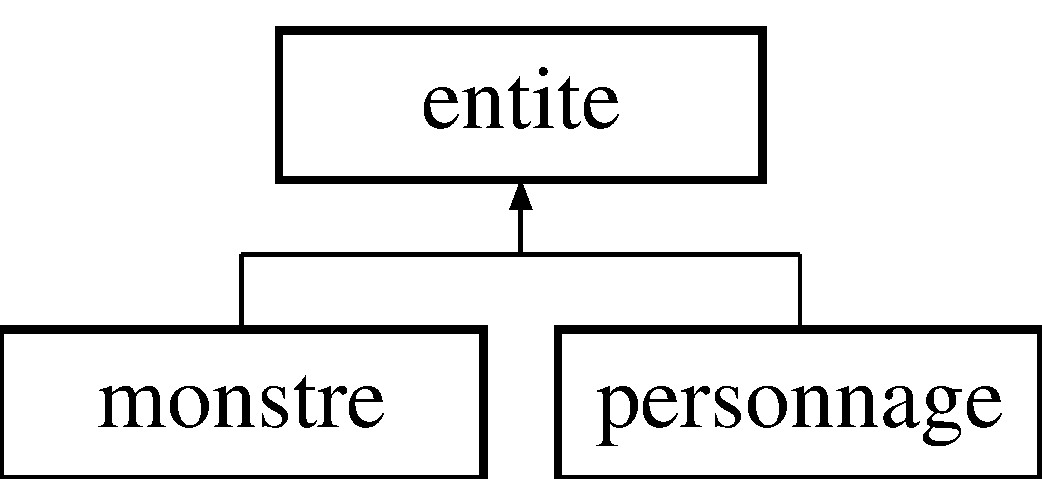
\includegraphics[height=2.000000cm]{classentite}
\end{center}
\end{figure}
\subsection*{Public Member Functions}
\begin{DoxyCompactItemize}
\item 
\hyperlink{classentite_a41b83303ba28a228fdfad7de3eed40fe}{entite} ()
\begin{DoxyCompactList}\small\item\em Constructeur vide. \end{DoxyCompactList}\item 
\hyperlink{classentite_a5e655b5c1999ae75dfca0b32de737b1e}{entite} (std\+::string \hyperlink{classentite_a904e8783de9fe2fc4306bf6b7822d025}{entite\+Id}, std\+::string \hyperlink{classentite_abe631a515b1cd0866dcfb078c4ceb07a}{entite\+Name}, int \hyperlink{classentite_a754557f56c1c1fcbcbd40eec68b60f65}{entite\+Hp\+Max}, int \hyperlink{classentite_ad9df70a9bb07f07b3ebf520941c3a35f}{entite\+Speed}, int \hyperlink{classentite_a696167d32c27b3b2a2fa6b473a888b18}{entite\+Mana\+Max}, std\+::string \hyperlink{classentite_a6fab1d9a04ade2cb97ec0904b12c82c9}{entite\+Description}, std\+::vector$<$ \hyperlink{classcompetence}{competence} $>$ all\+Skills)
\begin{DoxyCompactList}\small\item\em Constructeur avec tout. \end{DoxyCompactList}\item 
{\footnotesize template$<$typename T $>$ }\\std\+::string \hyperlink{classentite_ab77d3864b5cfed8364816e27b9eb7077}{to\+String} (const T \&valeur)
\item 
std\+::string \hyperlink{classentite_a3af765474e7f288752f24334d0fc6bbd}{get\+ID} ()
\begin{DoxyCompactList}\small\item\em Getter pour l\textquotesingle{}id. \end{DoxyCompactList}\item 
std\+::string \hyperlink{classentite_a0ebd43d682f234a39faa04bb34173d03}{get\+Name} ()
\begin{DoxyCompactList}\small\item\em Getter pour le nom. \end{DoxyCompactList}\item 
std\+::string \hyperlink{classentite_ab19b8d18b4d947c85063b2225bbb9144}{get\+Description} ()
\begin{DoxyCompactList}\small\item\em Getter pour la description. \end{DoxyCompactList}\item 
int \hyperlink{classentite_ab8e6c4dd900884cba5bec025f1e55999}{get\+Hp\+Max} ()
\begin{DoxyCompactList}\small\item\em Getter pour le nombre de points de vie max. \end{DoxyCompactList}\item 
int \hyperlink{classentite_ae41fa12581d2f94d5f6ae67fec4e56e9}{get\+Hp\+Current} ()
\begin{DoxyCompactList}\small\item\em Getter pour le nombre de points de vie actuels. \end{DoxyCompactList}\item 
int \hyperlink{classentite_ab97281eadee20e03fe497396439260c9}{get\+Speed} ()
\begin{DoxyCompactList}\small\item\em Getter pour la vitesse d\textquotesingle{}attaque de l\textquotesingle{}entite. \end{DoxyCompactList}\item 
bool \hyperlink{classentite_a5a39811eb0c12ae85a23f152c8ba6d58}{get\+Alive} ()
\begin{DoxyCompactList}\small\item\em Getter qui permet de savoir si l\textquotesingle{}entite est en vie. \end{DoxyCompactList}\item 
int \hyperlink{classentite_a427218420d74bdec1f79f93572ecf24a}{get\+Mana\+Max} ()
\begin{DoxyCompactList}\small\item\em Getter pour la mana maximum de l\textquotesingle{}entite. \end{DoxyCompactList}\item 
int \hyperlink{classentite_ad3e7a419d79d7d7e836243c4920703e3}{get\+Mana\+Current} ()
\begin{DoxyCompactList}\small\item\em Getter pour la mana actuelle de l\textquotesingle{}entite. \end{DoxyCompactList}\item 
std\+::vector$<$ \hyperlink{classcompetence}{competence} $>$ \hyperlink{classentite_a90c927665d7c0b7d6d5202604887e1e2}{get\+Skill\+Vect} ()
\begin{DoxyCompactList}\small\item\em Getter qui renvoie un vecteur (std\+::vector) de compétences. \end{DoxyCompactList}\item 
int \hyperlink{classentite_a983d51dcdfaaddaf95096587ea33a3ec}{nb\+Ligne\+Fichier} (std\+::string nom\+Fichier)
\begin{DoxyCompactList}\small\item\em Retour d\textquotesingle{}une string représentant un entite. \end{DoxyCompactList}\item 
std\+::string \hyperlink{classentite_aef8675e5f8592e0cc56661d4d5827d1f}{entite\+String} (std\+::string lettre\+Entite, std\+::string nom\+Fichier)
\item 
void \hyperlink{classentite_a7bd09aa63160345500b6d6c4dca6cf52}{save\+In\+File} (std\+::string lettre\+Entite, std\+::string nom\+Fichier)
\begin{DoxyCompactList}\small\item\em Permet d\textquotesingle{}écrire l\textquotesingle{}entite dans un fichier de sauvegarde. \end{DoxyCompactList}\item 
void \hyperlink{classentite_abb1bd724598359ea2b7c3b05546d59d3}{print\+Entite} ()
\begin{DoxyCompactList}\small\item\em Pour tester. \end{DoxyCompactList}\item 
bool \hyperlink{classentite_a024cbcffabd07556d550f5941f2113d4}{enlever\+Vie} (int degats)
\begin{DoxyCompactList}\small\item\em Enlève x points de vie a l\textquotesingle{}entite. \end{DoxyCompactList}\item 
bool \hyperlink{classentite_a48c1c38c58bbfa074885ac45a2584772}{enlever\+Mana} (int skill\+Mana\+Cost)
\begin{DoxyCompactList}\small\item\em Enlève x points de mana a l\textquotesingle{}entite. \end{DoxyCompactList}\end{DoxyCompactItemize}
\subsection*{Protected Attributes}
\begin{DoxyCompactItemize}
\item 
std\+::string \hyperlink{classentite_a904e8783de9fe2fc4306bf6b7822d025}{entite\+Id}
\item 
std\+::string \hyperlink{classentite_abe631a515b1cd0866dcfb078c4ceb07a}{entite\+Name}
\item 
std\+::string \hyperlink{classentite_a6fab1d9a04ade2cb97ec0904b12c82c9}{entite\+Description}
\item 
int \hyperlink{classentite_a754557f56c1c1fcbcbd40eec68b60f65}{entite\+Hp\+Max}
\item 
int \hyperlink{classentite_a09661bc80d898530a760153f6b690070}{entite\+Hp\+Current}
\item 
int \hyperlink{classentite_a696167d32c27b3b2a2fa6b473a888b18}{entite\+Mana\+Max}
\item 
int \hyperlink{classentite_ae194ea6eb360db3882fc0559a144899b}{entite\+Mana\+Current}
\item 
int \hyperlink{classentite_ad9df70a9bb07f07b3ebf520941c3a35f}{entite\+Speed}
\item 
bool \hyperlink{classentite_a5a69c21a4435817f2d960e0811d4474e}{entite\+Alive}
\item 
std\+::vector$<$ \hyperlink{classcompetence}{competence} $>$ \hyperlink{classentite_ad9d38b74abc49ec4fba0fcb27f4edaa9}{entite\+Skill\+Vect}
\end{DoxyCompactItemize}


\subsection{Constructor \& Destructor Documentation}
\mbox{\Hypertarget{classentite_a41b83303ba28a228fdfad7de3eed40fe}\label{classentite_a41b83303ba28a228fdfad7de3eed40fe}} 
\index{entite@{entite}!entite@{entite}}
\index{entite@{entite}!entite@{entite}}
\subsubsection{\texorpdfstring{entite()}{entite()}\hspace{0.1cm}{\footnotesize\ttfamily [1/2]}}
{\footnotesize\ttfamily entite\+::entite (\begin{DoxyParamCaption}{ }\end{DoxyParamCaption})}



Constructeur vide. 

\mbox{\Hypertarget{classentite_a5e655b5c1999ae75dfca0b32de737b1e}\label{classentite_a5e655b5c1999ae75dfca0b32de737b1e}} 
\index{entite@{entite}!entite@{entite}}
\index{entite@{entite}!entite@{entite}}
\subsubsection{\texorpdfstring{entite()}{entite()}\hspace{0.1cm}{\footnotesize\ttfamily [2/2]}}
{\footnotesize\ttfamily entite\+::entite (\begin{DoxyParamCaption}\item[{std\+::string}]{entite\+Id,  }\item[{std\+::string}]{entite\+Name,  }\item[{int}]{entite\+Hp\+Max,  }\item[{int}]{entite\+Speed,  }\item[{int}]{entite\+Mana\+Max,  }\item[{std\+::string}]{entite\+Description,  }\item[{std\+::vector$<$ \hyperlink{classcompetence}{competence} $>$}]{all\+Skills }\end{DoxyParamCaption})}



Constructeur avec tout. 


\begin{DoxyParams}{Parameters}
{\em entite\+Id} & L\textquotesingle{}identifiant de l\textquotesingle{}entite \\
\hline
{\em entite\+Name} & Le nom de l\textquotesingle{}entite \\
\hline
{\em entite\+Hp\+Max} & Les points de vie max de l\textquotesingle{}entite \\
\hline
{\em entite\+Speed} & La vitesse de l\textquotesingle{}entite \\
\hline
{\em entite\+Mana\+Max} & Les points de mana max de l\textquotesingle{}entite \\
\hline
{\em entite\+Description} & La description de l\textquotesingle{}entite \\
\hline
{\em all\+Skills} & Un vecteur (std\+::vector) contenant toutes les compétences de cette entite. \\
\hline
\end{DoxyParams}


\subsection{Member Function Documentation}
\mbox{\Hypertarget{classentite_a48c1c38c58bbfa074885ac45a2584772}\label{classentite_a48c1c38c58bbfa074885ac45a2584772}} 
\index{entite@{entite}!enlever\+Mana@{enlever\+Mana}}
\index{enlever\+Mana@{enlever\+Mana}!entite@{entite}}
\subsubsection{\texorpdfstring{enlever\+Mana()}{enleverMana()}}
{\footnotesize\ttfamily bool entite\+::enlever\+Mana (\begin{DoxyParamCaption}\item[{int}]{skill\+Mana\+Cost }\end{DoxyParamCaption})}



Enlève x points de mana a l\textquotesingle{}entite. 

Cette fonction ne sert à rien, à part ne pas faire bugger les autres. \begin{DoxyReturn}{Returns}
Un booléen vérifiant la capacité à dépenser la mana. 
\end{DoxyReturn}
\mbox{\Hypertarget{classentite_a024cbcffabd07556d550f5941f2113d4}\label{classentite_a024cbcffabd07556d550f5941f2113d4}} 
\index{entite@{entite}!enlever\+Vie@{enlever\+Vie}}
\index{enlever\+Vie@{enlever\+Vie}!entite@{entite}}
\subsubsection{\texorpdfstring{enlever\+Vie()}{enleverVie()}}
{\footnotesize\ttfamily bool entite\+::enlever\+Vie (\begin{DoxyParamCaption}\item[{int}]{degats }\end{DoxyParamCaption})}



Enlève x points de vie a l\textquotesingle{}entite. 

Cette fonction permet d\textquotesingle{}enlever des points de vie. Elle permet aussi de savoir si une entite est en vie (pts\+Vie $<$ 0) ou si elle est morte. \begin{DoxyReturn}{Returns}
Un booléen qui est égal à {\ttfamily true} si le entite est mort, {\ttfamily false} sinon. 
\end{DoxyReturn}
\mbox{\Hypertarget{classentite_aef8675e5f8592e0cc56661d4d5827d1f}\label{classentite_aef8675e5f8592e0cc56661d4d5827d1f}} 
\index{entite@{entite}!entite\+String@{entite\+String}}
\index{entite\+String@{entite\+String}!entite@{entite}}
\subsubsection{\texorpdfstring{entite\+String()}{entiteString()}}
{\footnotesize\ttfamily std\+::string entite\+::entite\+String (\begin{DoxyParamCaption}\item[{std\+::string}]{lettre\+Entite,  }\item[{std\+::string}]{nom\+Fichier }\end{DoxyParamCaption})}

\mbox{\Hypertarget{classentite_a5a39811eb0c12ae85a23f152c8ba6d58}\label{classentite_a5a39811eb0c12ae85a23f152c8ba6d58}} 
\index{entite@{entite}!get\+Alive@{get\+Alive}}
\index{get\+Alive@{get\+Alive}!entite@{entite}}
\subsubsection{\texorpdfstring{get\+Alive()}{getAlive()}}
{\footnotesize\ttfamily bool entite\+::get\+Alive (\begin{DoxyParamCaption}{ }\end{DoxyParamCaption})}



Getter qui permet de savoir si l\textquotesingle{}entite est en vie. 

\mbox{\Hypertarget{classentite_ab19b8d18b4d947c85063b2225bbb9144}\label{classentite_ab19b8d18b4d947c85063b2225bbb9144}} 
\index{entite@{entite}!get\+Description@{get\+Description}}
\index{get\+Description@{get\+Description}!entite@{entite}}
\subsubsection{\texorpdfstring{get\+Description()}{getDescription()}}
{\footnotesize\ttfamily std\+::string entite\+::get\+Description (\begin{DoxyParamCaption}{ }\end{DoxyParamCaption})}



Getter pour la description. 

\mbox{\Hypertarget{classentite_ae41fa12581d2f94d5f6ae67fec4e56e9}\label{classentite_ae41fa12581d2f94d5f6ae67fec4e56e9}} 
\index{entite@{entite}!get\+Hp\+Current@{get\+Hp\+Current}}
\index{get\+Hp\+Current@{get\+Hp\+Current}!entite@{entite}}
\subsubsection{\texorpdfstring{get\+Hp\+Current()}{getHpCurrent()}}
{\footnotesize\ttfamily int entite\+::get\+Hp\+Current (\begin{DoxyParamCaption}{ }\end{DoxyParamCaption})}



Getter pour le nombre de points de vie actuels. 

\mbox{\Hypertarget{classentite_ab8e6c4dd900884cba5bec025f1e55999}\label{classentite_ab8e6c4dd900884cba5bec025f1e55999}} 
\index{entite@{entite}!get\+Hp\+Max@{get\+Hp\+Max}}
\index{get\+Hp\+Max@{get\+Hp\+Max}!entite@{entite}}
\subsubsection{\texorpdfstring{get\+Hp\+Max()}{getHpMax()}}
{\footnotesize\ttfamily int entite\+::get\+Hp\+Max (\begin{DoxyParamCaption}{ }\end{DoxyParamCaption})}



Getter pour le nombre de points de vie max. 

\mbox{\Hypertarget{classentite_a3af765474e7f288752f24334d0fc6bbd}\label{classentite_a3af765474e7f288752f24334d0fc6bbd}} 
\index{entite@{entite}!get\+ID@{get\+ID}}
\index{get\+ID@{get\+ID}!entite@{entite}}
\subsubsection{\texorpdfstring{get\+I\+D()}{getID()}}
{\footnotesize\ttfamily std\+::string entite\+::get\+ID (\begin{DoxyParamCaption}{ }\end{DoxyParamCaption})}



Getter pour l\textquotesingle{}id. 

\mbox{\Hypertarget{classentite_ad3e7a419d79d7d7e836243c4920703e3}\label{classentite_ad3e7a419d79d7d7e836243c4920703e3}} 
\index{entite@{entite}!get\+Mana\+Current@{get\+Mana\+Current}}
\index{get\+Mana\+Current@{get\+Mana\+Current}!entite@{entite}}
\subsubsection{\texorpdfstring{get\+Mana\+Current()}{getManaCurrent()}}
{\footnotesize\ttfamily int entite\+::get\+Mana\+Current (\begin{DoxyParamCaption}{ }\end{DoxyParamCaption})}



Getter pour la mana actuelle de l\textquotesingle{}entite. 

\mbox{\Hypertarget{classentite_a427218420d74bdec1f79f93572ecf24a}\label{classentite_a427218420d74bdec1f79f93572ecf24a}} 
\index{entite@{entite}!get\+Mana\+Max@{get\+Mana\+Max}}
\index{get\+Mana\+Max@{get\+Mana\+Max}!entite@{entite}}
\subsubsection{\texorpdfstring{get\+Mana\+Max()}{getManaMax()}}
{\footnotesize\ttfamily int entite\+::get\+Mana\+Max (\begin{DoxyParamCaption}{ }\end{DoxyParamCaption})}



Getter pour la mana maximum de l\textquotesingle{}entite. 

\mbox{\Hypertarget{classentite_a0ebd43d682f234a39faa04bb34173d03}\label{classentite_a0ebd43d682f234a39faa04bb34173d03}} 
\index{entite@{entite}!get\+Name@{get\+Name}}
\index{get\+Name@{get\+Name}!entite@{entite}}
\subsubsection{\texorpdfstring{get\+Name()}{getName()}}
{\footnotesize\ttfamily std\+::string entite\+::get\+Name (\begin{DoxyParamCaption}{ }\end{DoxyParamCaption})}



Getter pour le nom. 

\mbox{\Hypertarget{classentite_a90c927665d7c0b7d6d5202604887e1e2}\label{classentite_a90c927665d7c0b7d6d5202604887e1e2}} 
\index{entite@{entite}!get\+Skill\+Vect@{get\+Skill\+Vect}}
\index{get\+Skill\+Vect@{get\+Skill\+Vect}!entite@{entite}}
\subsubsection{\texorpdfstring{get\+Skill\+Vect()}{getSkillVect()}}
{\footnotesize\ttfamily std\+::vector$<$\hyperlink{classcompetence}{competence}$>$ entite\+::get\+Skill\+Vect (\begin{DoxyParamCaption}{ }\end{DoxyParamCaption})}



Getter qui renvoie un vecteur (std\+::vector) de compétences. 

\mbox{\Hypertarget{classentite_ab97281eadee20e03fe497396439260c9}\label{classentite_ab97281eadee20e03fe497396439260c9}} 
\index{entite@{entite}!get\+Speed@{get\+Speed}}
\index{get\+Speed@{get\+Speed}!entite@{entite}}
\subsubsection{\texorpdfstring{get\+Speed()}{getSpeed()}}
{\footnotesize\ttfamily int entite\+::get\+Speed (\begin{DoxyParamCaption}{ }\end{DoxyParamCaption})}



Getter pour la vitesse d\textquotesingle{}attaque de l\textquotesingle{}entite. 

\mbox{\Hypertarget{classentite_a983d51dcdfaaddaf95096587ea33a3ec}\label{classentite_a983d51dcdfaaddaf95096587ea33a3ec}} 
\index{entite@{entite}!nb\+Ligne\+Fichier@{nb\+Ligne\+Fichier}}
\index{nb\+Ligne\+Fichier@{nb\+Ligne\+Fichier}!entite@{entite}}
\subsubsection{\texorpdfstring{nb\+Ligne\+Fichier()}{nbLigneFichier()}}
{\footnotesize\ttfamily int entite\+::nb\+Ligne\+Fichier (\begin{DoxyParamCaption}\item[{std\+::string}]{nom\+Fichier }\end{DoxyParamCaption})}



Retour d\textquotesingle{}une string représentant un entite. 

Convertit un objet entite en une ligne de string. \begin{DoxyPostcond}{Postcondition}
La string contiendra les infos dans cet ordre \+:
\begin{DoxyItemize}
\item entite\+Identifiant (type {\ttfamily m$<$entier$>$})
\item nom de l\textquotesingle{}entite
\item nombre de points de vie
\item vitesse d\textquotesingle{}attaque
\item toutes les compétences , séparées par des {\ttfamily \+:}Retourne le nombre de lignes d\textquotesingle{}un fichier.
\end{DoxyItemize}
\end{DoxyPostcond}
Compte le nb de lignes du fichier pour créer l\textquotesingle{}identifiant unique d\textquotesingle{}un entite. L\textquotesingle{}identifiant sera {\ttfamily  nb\+Lignes + 1 } \begin{DoxyReturn}{Returns}
Un entier représentant le nombre de lignes. 
\end{DoxyReturn}

\begin{DoxyParams}{Parameters}
{\em nom\+Fichier} & Une string (std\+::string) qui sera le nom du fichier à ouvrir. \\
\hline
\end{DoxyParams}
\mbox{\Hypertarget{classentite_abb1bd724598359ea2b7c3b05546d59d3}\label{classentite_abb1bd724598359ea2b7c3b05546d59d3}} 
\index{entite@{entite}!print\+Entite@{print\+Entite}}
\index{print\+Entite@{print\+Entite}!entite@{entite}}
\subsubsection{\texorpdfstring{print\+Entite()}{printEntite()}}
{\footnotesize\ttfamily void entite\+::print\+Entite (\begin{DoxyParamCaption}{ }\end{DoxyParamCaption})}



Pour tester. 

\mbox{\Hypertarget{classentite_a7bd09aa63160345500b6d6c4dca6cf52}\label{classentite_a7bd09aa63160345500b6d6c4dca6cf52}} 
\index{entite@{entite}!save\+In\+File@{save\+In\+File}}
\index{save\+In\+File@{save\+In\+File}!entite@{entite}}
\subsubsection{\texorpdfstring{save\+In\+File()}{saveInFile()}}
{\footnotesize\ttfamily void entite\+::save\+In\+File (\begin{DoxyParamCaption}\item[{std\+::string}]{lettre\+Entite,  }\item[{std\+::string}]{nom\+Fichier }\end{DoxyParamCaption})}



Permet d\textquotesingle{}écrire l\textquotesingle{}entite dans un fichier de sauvegarde. 

\mbox{\Hypertarget{classentite_ab77d3864b5cfed8364816e27b9eb7077}\label{classentite_ab77d3864b5cfed8364816e27b9eb7077}} 
\index{entite@{entite}!to\+String@{to\+String}}
\index{to\+String@{to\+String}!entite@{entite}}
\subsubsection{\texorpdfstring{to\+String()}{toString()}}
{\footnotesize\ttfamily template$<$typename T $>$ \\
std\+::string entite\+::to\+String (\begin{DoxyParamCaption}\item[{const T \&}]{valeur }\end{DoxyParamCaption})}



\subsection{Member Data Documentation}
\mbox{\Hypertarget{classentite_a5a69c21a4435817f2d960e0811d4474e}\label{classentite_a5a69c21a4435817f2d960e0811d4474e}} 
\index{entite@{entite}!entite\+Alive@{entite\+Alive}}
\index{entite\+Alive@{entite\+Alive}!entite@{entite}}
\subsubsection{\texorpdfstring{entite\+Alive}{entiteAlive}}
{\footnotesize\ttfamily bool entite\+::entite\+Alive\hspace{0.3cm}{\ttfamily [protected]}}

\mbox{\Hypertarget{classentite_a6fab1d9a04ade2cb97ec0904b12c82c9}\label{classentite_a6fab1d9a04ade2cb97ec0904b12c82c9}} 
\index{entite@{entite}!entite\+Description@{entite\+Description}}
\index{entite\+Description@{entite\+Description}!entite@{entite}}
\subsubsection{\texorpdfstring{entite\+Description}{entiteDescription}}
{\footnotesize\ttfamily std\+::string entite\+::entite\+Description\hspace{0.3cm}{\ttfamily [protected]}}

\mbox{\Hypertarget{classentite_a09661bc80d898530a760153f6b690070}\label{classentite_a09661bc80d898530a760153f6b690070}} 
\index{entite@{entite}!entite\+Hp\+Current@{entite\+Hp\+Current}}
\index{entite\+Hp\+Current@{entite\+Hp\+Current}!entite@{entite}}
\subsubsection{\texorpdfstring{entite\+Hp\+Current}{entiteHpCurrent}}
{\footnotesize\ttfamily int entite\+::entite\+Hp\+Current\hspace{0.3cm}{\ttfamily [protected]}}

\mbox{\Hypertarget{classentite_a754557f56c1c1fcbcbd40eec68b60f65}\label{classentite_a754557f56c1c1fcbcbd40eec68b60f65}} 
\index{entite@{entite}!entite\+Hp\+Max@{entite\+Hp\+Max}}
\index{entite\+Hp\+Max@{entite\+Hp\+Max}!entite@{entite}}
\subsubsection{\texorpdfstring{entite\+Hp\+Max}{entiteHpMax}}
{\footnotesize\ttfamily int entite\+::entite\+Hp\+Max\hspace{0.3cm}{\ttfamily [protected]}}

\mbox{\Hypertarget{classentite_a904e8783de9fe2fc4306bf6b7822d025}\label{classentite_a904e8783de9fe2fc4306bf6b7822d025}} 
\index{entite@{entite}!entite\+Id@{entite\+Id}}
\index{entite\+Id@{entite\+Id}!entite@{entite}}
\subsubsection{\texorpdfstring{entite\+Id}{entiteId}}
{\footnotesize\ttfamily std\+::string entite\+::entite\+Id\hspace{0.3cm}{\ttfamily [protected]}}

\mbox{\Hypertarget{classentite_ae194ea6eb360db3882fc0559a144899b}\label{classentite_ae194ea6eb360db3882fc0559a144899b}} 
\index{entite@{entite}!entite\+Mana\+Current@{entite\+Mana\+Current}}
\index{entite\+Mana\+Current@{entite\+Mana\+Current}!entite@{entite}}
\subsubsection{\texorpdfstring{entite\+Mana\+Current}{entiteManaCurrent}}
{\footnotesize\ttfamily int entite\+::entite\+Mana\+Current\hspace{0.3cm}{\ttfamily [protected]}}

\mbox{\Hypertarget{classentite_a696167d32c27b3b2a2fa6b473a888b18}\label{classentite_a696167d32c27b3b2a2fa6b473a888b18}} 
\index{entite@{entite}!entite\+Mana\+Max@{entite\+Mana\+Max}}
\index{entite\+Mana\+Max@{entite\+Mana\+Max}!entite@{entite}}
\subsubsection{\texorpdfstring{entite\+Mana\+Max}{entiteManaMax}}
{\footnotesize\ttfamily int entite\+::entite\+Mana\+Max\hspace{0.3cm}{\ttfamily [protected]}}

\mbox{\Hypertarget{classentite_abe631a515b1cd0866dcfb078c4ceb07a}\label{classentite_abe631a515b1cd0866dcfb078c4ceb07a}} 
\index{entite@{entite}!entite\+Name@{entite\+Name}}
\index{entite\+Name@{entite\+Name}!entite@{entite}}
\subsubsection{\texorpdfstring{entite\+Name}{entiteName}}
{\footnotesize\ttfamily std\+::string entite\+::entite\+Name\hspace{0.3cm}{\ttfamily [protected]}}

\mbox{\Hypertarget{classentite_ad9d38b74abc49ec4fba0fcb27f4edaa9}\label{classentite_ad9d38b74abc49ec4fba0fcb27f4edaa9}} 
\index{entite@{entite}!entite\+Skill\+Vect@{entite\+Skill\+Vect}}
\index{entite\+Skill\+Vect@{entite\+Skill\+Vect}!entite@{entite}}
\subsubsection{\texorpdfstring{entite\+Skill\+Vect}{entiteSkillVect}}
{\footnotesize\ttfamily std\+::vector$<$\hyperlink{classcompetence}{competence}$>$ entite\+::entite\+Skill\+Vect\hspace{0.3cm}{\ttfamily [protected]}}

\mbox{\Hypertarget{classentite_ad9df70a9bb07f07b3ebf520941c3a35f}\label{classentite_ad9df70a9bb07f07b3ebf520941c3a35f}} 
\index{entite@{entite}!entite\+Speed@{entite\+Speed}}
\index{entite\+Speed@{entite\+Speed}!entite@{entite}}
\subsubsection{\texorpdfstring{entite\+Speed}{entiteSpeed}}
{\footnotesize\ttfamily int entite\+::entite\+Speed\hspace{0.3cm}{\ttfamily [protected]}}



The documentation for this class was generated from the following file\+:\begin{DoxyCompactItemize}
\item 
/\+Users/thibault/\+Git\+Hub/\+C\+E\+R\+I\+\_\+software\+\_\+engineering\+\_\+game\+\_\+1/headers/\hyperlink{entite_8h}{entite.\+h}\end{DoxyCompactItemize}

\hypertarget{classjeu}{}\section{jeu Class Reference}
\label{classjeu}\index{jeu@{jeu}}


Ceci sera la classe du jeu. Elle contient toutes les entités, la carte, ainsi que les fonctions nécessaires à la partie.  




{\ttfamily \#include $<$fonctionsjeu.\+h$>$}

\subsection*{Public Member Functions}
\begin{DoxyCompactItemize}
\item 
\hyperlink{classjeu_a38513a7bfd0a7ea4e3a5612da2856016}{jeu} ()
\begin{DoxyCompactList}\small\item\em Temporaire!! \end{DoxyCompactList}\item 
\hyperlink{classjeu_a55385a33ef40e0579eb3a3634566c4a8}{$\sim$jeu} ()
\begin{DoxyCompactList}\small\item\em Destructeur par défaut. \end{DoxyCompactList}\item 
\hyperlink{class_carte}{Carte} \hyperlink{classjeu_ae2e46e1fdeb23fc643ed506b0df7f21f}{get\+Carte} ()
\begin{DoxyCompactList}\small\item\em Getter de carte de jeu. \end{DoxyCompactList}\item 
\hyperlink{classpersonnage}{personnage} \hyperlink{classjeu_a8bd58d1469db0d7595bb732403036823}{get\+Perso} ()
\begin{DoxyCompactList}\small\item\em Getter de personnage. \end{DoxyCompactList}\item 
std\+::vector$<$ \hyperlink{classmonstre}{monstre} $>$ \hyperlink{classjeu_a22e7a7e7b932b935fa73658820038176}{get\+Monstres} ()
\begin{DoxyCompactList}\small\item\em Getter de vecteur de monstres. \end{DoxyCompactList}\item 
int \hyperlink{classjeu_ae172cfaf3e5c97e1576dc4069d48ec94}{get\+Nb\+Monstres} ()
\begin{DoxyCompactList}\small\item\em Getter de nombre de monstres. \end{DoxyCompactList}\item 
void \hyperlink{classjeu_a53cb5e2a1c7e0925aca09885ff959efc}{set\+Jeu\+Carte} (\hyperlink{class_carte}{Carte} jeu\+\_\+map)
\begin{DoxyCompactList}\small\item\em Setter de carte de jeu. \end{DoxyCompactList}\item 
void \hyperlink{classjeu_a852b0a8b2d17f0af120c6798861ef806}{deplacement} (int \&result)
\begin{DoxyCompactList}\small\item\em Fonction de déplacement du joueur sur la carte. \end{DoxyCompactList}\item 
void \hyperlink{classjeu_a834e8a14bd0324c88b2de777a6bdf30f}{afficher\+Jeu} (int \&result)
\begin{DoxyCompactList}\small\item\em Fonction permettant d\textquotesingle{}afficher la carte, puis de demander un déplacement au joueur. \end{DoxyCompactList}\item 
std\+::string \hyperlink{classjeu_a58d74300f8d64b3d3cd151e0838ef232}{generer\+Deplacement} (std\+::vector$<$ bool $>$ \&v)
\begin{DoxyCompactList}\small\item\em Fonction permettant de générer les déplacements possibles à partir d\textquotesingle{}une case {\ttfamily i,j} du plateau de jeu. \end{DoxyCompactList}\item 
std\+::string \hyperlink{classjeu_ae186e98661e72378c9e659ffcf7a7deb}{generer\+Input\+Accepte} (std\+::vector$<$ bool $>$ b)
\begin{DoxyCompactList}\small\item\em Fonction permettant de générer une chaine d\textquotesingle{}entrées utilisateur acceptables pour le déplacement. \end{DoxyCompactList}\item 
int \hyperlink{classjeu_aa96615463266652e0bdc685c9afe5cfe}{combat} (std\+::string id\+\_\+monstre)
\begin{DoxyCompactList}\small\item\em Module de combat. \end{DoxyCompactList}\item 
std\+::vector$<$ \hyperlink{classmonstre}{monstre} $>$\+::iterator \hyperlink{classjeu_af3a81d9b899b204b4b304821c5bee43b}{cherche\+\_\+monstre} (std\+::string id\+\_\+monstre)
\begin{DoxyCompactList}\small\item\em Recherche de monstre. \end{DoxyCompactList}\item 
bool \hyperlink{classjeu_a77728b27a5a1f4194ac77c414b983f01}{chargement\+\_\+entite} (std\+::vector$<$ \hyperlink{classentite}{entite} $>$ \&vect\+\_\+entite, std\+::string id\+\_\+monstre)
\begin{DoxyCompactList}\small\item\em Chargement acteurs combat. \end{DoxyCompactList}\item 
std\+::vector$<$ int $>$ \hyperlink{classjeu_afd7a155c8adcee663d6aeb98b2dae010}{orga\+\_\+entites} (std\+::vector$<$ \hyperlink{classentite}{entite} $>$ \&vect\+\_\+entite)
\begin{DoxyCompactList}\small\item\em Organisation entités. \end{DoxyCompactList}\item 
\hyperlink{classcompetence}{competence} \hyperlink{classjeu_a91981b755a6b0895703d9adf537f0ae6}{choix\+\_\+comp} (\hyperlink{classentite}{entite} \&indiv)
\begin{DoxyCompactList}\small\item\em Choix compétence. \end{DoxyCompactList}\item 
\hyperlink{classentite}{entite} \hyperlink{classjeu_ad9ea0cb9e74e6d9b0385720528450f61}{choix\+\_\+target} (\hyperlink{classcompetence}{competence} comp\+\_\+util, \hyperlink{classentite}{entite} \&indiv, std\+::vector$<$ \hyperlink{classentite}{entite} $>$ \&vect\+\_\+entite, std\+::vector$<$ int $>$ vect\+\_\+p)
\begin{DoxyCompactList}\small\item\em Choix cible. \end{DoxyCompactList}\item 
int \hyperlink{classjeu_a6bc1f7cfd93bdc33fc9f841ec3f5f80f}{appliquer\+\_\+comp} (\hyperlink{classentite}{entite} indiv, \hyperlink{classentite}{entite} target, std\+::vector$<$ \hyperlink{classentite}{entite} $>$ \&vect\+\_\+entite, \hyperlink{classcompetence}{competence} comp\+\_\+util, int \&nb\+\_\+players, int \&nb\+\_\+monsters)
\begin{DoxyCompactList}\small\item\em Appliquer compétence. \end{DoxyCompactList}\item 
void \hyperlink{classjeu_a110399c4103d3d4391f2007856c3e009}{quit\+Game} ()
\begin{DoxyCompactList}\small\item\em Quitte le jeu, sans que l\textquotesingle{}utilisateur n\textquotesingle{}ai gagné ni perdu. \end{DoxyCompactList}\item 
void \hyperlink{classjeu_a7c769fff9b23935aef40d6633d774a96}{victoire\+Game} ()
\begin{DoxyCompactList}\small\item\em Affiche un message de victoire à l\textquotesingle{}utilisateur. \end{DoxyCompactList}\item 
void \hyperlink{classjeu_aa6163ba51f80fa944374fc1b85021268}{failed\+Game} ()
\begin{DoxyCompactList}\small\item\em Affiche un message de défait au joueur. \end{DoxyCompactList}\end{DoxyCompactItemize}


\subsection{Detailed Description}
Ceci sera la classe du jeu. Elle contient toutes les entités, la carte, ainsi que les fonctions nécessaires à la partie. 

Cette classe contient les fonctions nécessaires au démarrage de la partie, au combat, ainsi que toutes les fonctions intermédiaires nécessaires au bon fonctionnement de celles-\/ci.

Inclut la librairie io. 

\subsection{Constructor \& Destructor Documentation}
\mbox{\Hypertarget{classjeu_a38513a7bfd0a7ea4e3a5612da2856016}\label{classjeu_a38513a7bfd0a7ea4e3a5612da2856016}} 
\index{jeu@{jeu}!jeu@{jeu}}
\index{jeu@{jeu}!jeu@{jeu}}
\subsubsection{\texorpdfstring{jeu()}{jeu()}}
{\footnotesize\ttfamily jeu\+::jeu (\begin{DoxyParamCaption}{ }\end{DoxyParamCaption})}



Temporaire!! 

Constructeur par défaut sans argument.

Affichage d\textquotesingle{}un message de bienvenue. Choix du personnage. Choix de la carte. Chargement des monstres.

\begin{DoxySeeAlso}{See also}
perso(), carte(), \hyperlink{classmonstre}{monstre()} 
\end{DoxySeeAlso}
\mbox{\Hypertarget{classjeu_a55385a33ef40e0579eb3a3634566c4a8}\label{classjeu_a55385a33ef40e0579eb3a3634566c4a8}} 
\index{jeu@{jeu}!````~jeu@{$\sim$jeu}}
\index{````~jeu@{$\sim$jeu}!jeu@{jeu}}
\subsubsection{\texorpdfstring{$\sim$jeu()}{~jeu()}}
{\footnotesize\ttfamily jeu\+::$\sim$jeu (\begin{DoxyParamCaption}{ }\end{DoxyParamCaption})}



Destructeur par défaut. 



\subsection{Member Function Documentation}
\mbox{\Hypertarget{classjeu_a834e8a14bd0324c88b2de777a6bdf30f}\label{classjeu_a834e8a14bd0324c88b2de777a6bdf30f}} 
\index{jeu@{jeu}!afficher\+Jeu@{afficher\+Jeu}}
\index{afficher\+Jeu@{afficher\+Jeu}!jeu@{jeu}}
\subsubsection{\texorpdfstring{afficher\+Jeu()}{afficherJeu()}}
{\footnotesize\ttfamily void jeu\+::afficher\+Jeu (\begin{DoxyParamCaption}\item[{int \&}]{result }\end{DoxyParamCaption})}



Fonction permettant d\textquotesingle{}afficher la carte, puis de demander un déplacement au joueur. 

\begin{DoxyNote}{Note}
Cette fonction est là uniquement pour des fins de tests. La fonctionnalité qu\textquotesingle{}elle remplit sera remplacée par d\textquotesingle{}autres méthodes dans la fichier {\ttfamily tests/main.\+cpp}. 
\end{DoxyNote}
\mbox{\Hypertarget{classjeu_a6bc1f7cfd93bdc33fc9f841ec3f5f80f}\label{classjeu_a6bc1f7cfd93bdc33fc9f841ec3f5f80f}} 
\index{jeu@{jeu}!appliquer\+\_\+comp@{appliquer\+\_\+comp}}
\index{appliquer\+\_\+comp@{appliquer\+\_\+comp}!jeu@{jeu}}
\subsubsection{\texorpdfstring{appliquer\+\_\+comp()}{appliquer\_comp()}}
{\footnotesize\ttfamily int jeu\+::appliquer\+\_\+comp (\begin{DoxyParamCaption}\item[{\hyperlink{classentite}{entite}}]{indiv,  }\item[{\hyperlink{classentite}{entite}}]{target,  }\item[{std\+::vector$<$ \hyperlink{classentite}{entite} $>$ \&}]{vect\+\_\+entite,  }\item[{\hyperlink{classcompetence}{competence}}]{comp\+\_\+util,  }\item[{int \&}]{nb\+\_\+players,  }\item[{int \&}]{nb\+\_\+monsters }\end{DoxyParamCaption})}



Appliquer compétence. 

Permet d\textquotesingle{}appliquer les effets de la compétence choisie sur la cible choisie. Si la cible meurt, décrémente le compteur de personnages/monstres vivants. Supprime les cibles mortes du vecteur d\textquotesingle{}entités. 
\begin{DoxyParams}{Parameters}
{\em target} & Cible de la compétence. \\
\hline
{\em vect\+\_\+entite} & Le vecteur duquel on tire la cible de la compétence. \\
\hline
{\em comp\+\_\+util} & La compétence à utiliser. \\
\hline
{\em nb\+\_\+players} & Le nombre total de joueurs de la partie. \\
\hline
{\em nb\+\_\+monsters} & Le nombre de monstres du combat en cours. \\
\hline
\end{DoxyParams}
\begin{DoxyReturn}{Returns}
Un entier\+: 1 si tous les monstres sont morts, 0 si tous les joueurs sont morts, 2 sinon. 
\end{DoxyReturn}
\begin{DoxySeeAlso}{See also}
enlever\+Vie() 
\end{DoxySeeAlso}
\mbox{\Hypertarget{classjeu_a77728b27a5a1f4194ac77c414b983f01}\label{classjeu_a77728b27a5a1f4194ac77c414b983f01}} 
\index{jeu@{jeu}!chargement\+\_\+entite@{chargement\+\_\+entite}}
\index{chargement\+\_\+entite@{chargement\+\_\+entite}!jeu@{jeu}}
\subsubsection{\texorpdfstring{chargement\+\_\+entite()}{chargement\_entite()}}
{\footnotesize\ttfamily bool jeu\+::chargement\+\_\+entite (\begin{DoxyParamCaption}\item[{std\+::vector$<$ \hyperlink{classentite}{entite} $>$ \&}]{vect\+\_\+entite,  }\item[{std\+::string}]{id\+\_\+monstre }\end{DoxyParamCaption})}



Chargement acteurs combat. 

Permet de charger tous les acteurs du combat dans un vecteur d\textquotesingle{}entités. 
\begin{DoxyParams}{Parameters}
{\em vect\+\_\+entite} & Vecteur où chercher le monstre. \\
\hline
{\em id\+\_\+monstre} & Identifiant du monstre à charger. \\
\hline
\end{DoxyParams}
\begin{DoxyReturn}{Returns}
Chargement réussi ou non. 
\end{DoxyReturn}
\begin{DoxySeeAlso}{See also}
\hyperlink{classjeu_af3a81d9b899b204b4b304821c5bee43b}{cherche\+\_\+monstre()} 
\end{DoxySeeAlso}
\mbox{\Hypertarget{classjeu_af3a81d9b899b204b4b304821c5bee43b}\label{classjeu_af3a81d9b899b204b4b304821c5bee43b}} 
\index{jeu@{jeu}!cherche\+\_\+monstre@{cherche\+\_\+monstre}}
\index{cherche\+\_\+monstre@{cherche\+\_\+monstre}!jeu@{jeu}}
\subsubsection{\texorpdfstring{cherche\+\_\+monstre()}{cherche\_monstre()}}
{\footnotesize\ttfamily std\+::vector$<$\hyperlink{classmonstre}{monstre}$>$\+::iterator jeu\+::cherche\+\_\+monstre (\begin{DoxyParamCaption}\item[{std\+::string}]{id\+\_\+monstre }\end{DoxyParamCaption})}



Recherche de monstre. 

Permet de trouver l\textquotesingle{}objet monstre correspondant à la string id trouvée sur une case. Si la valeur renvoyée correspond à la fin du vecteur, le monstre n\textquotesingle{}a pas été trouvé. 
\begin{DoxyParams}{Parameters}
{\em id\+\_\+monstre} & Identifiant du monstre à trouver. \\
\hline
\end{DoxyParams}
\begin{DoxyReturn}{Returns}
Un itérateur correspondant à l\textquotesingle{}élément du vecteur de monstres concerné. 
\end{DoxyReturn}
\mbox{\Hypertarget{classjeu_a91981b755a6b0895703d9adf537f0ae6}\label{classjeu_a91981b755a6b0895703d9adf537f0ae6}} 
\index{jeu@{jeu}!choix\+\_\+comp@{choix\+\_\+comp}}
\index{choix\+\_\+comp@{choix\+\_\+comp}!jeu@{jeu}}
\subsubsection{\texorpdfstring{choix\+\_\+comp()}{choix\_comp()}}
{\footnotesize\ttfamily \hyperlink{classcompetence}{competence} jeu\+::choix\+\_\+comp (\begin{DoxyParamCaption}\item[{\hyperlink{classentite}{entite} \&}]{indiv }\end{DoxyParamCaption})}



Choix compétence. 

Permet de sélectionner une compétence par input parmi une liste tirée d\textquotesingle{}un vecteur (spécifique à chaque entité) Vérifie la possibilité du lancer (niveau de mana). Si l\textquotesingle{}entité est un monstre, le choix est aléatoire. 
\begin{DoxyParams}{Parameters}
{\em indiv} & L\textquotesingle{}entité qui joue actuellement. \\
\hline
\end{DoxyParams}
\begin{DoxyReturn}{Returns}
Une compétence parmi les compétences utilisables. 
\end{DoxyReturn}
\begin{DoxySeeAlso}{See also}
\hyperlink{namespaceio_ad045ca63d3481c2da3253a3944df18e4}{choix\+\_\+unique\+\_\+element()} 
\end{DoxySeeAlso}
\mbox{\Hypertarget{classjeu_ad9ea0cb9e74e6d9b0385720528450f61}\label{classjeu_ad9ea0cb9e74e6d9b0385720528450f61}} 
\index{jeu@{jeu}!choix\+\_\+target@{choix\+\_\+target}}
\index{choix\+\_\+target@{choix\+\_\+target}!jeu@{jeu}}
\subsubsection{\texorpdfstring{choix\+\_\+target()}{choix\_target()}}
{\footnotesize\ttfamily \hyperlink{classentite}{entite} jeu\+::choix\+\_\+target (\begin{DoxyParamCaption}\item[{\hyperlink{classcompetence}{competence}}]{comp\+\_\+util,  }\item[{\hyperlink{classentite}{entite} \&}]{indiv,  }\item[{std\+::vector$<$ \hyperlink{classentite}{entite} $>$ \&}]{vect\+\_\+entite,  }\item[{std\+::vector$<$ int $>$}]{vect\+\_\+p }\end{DoxyParamCaption})}



Choix cible. 

Permet de choisir une cible parmi une liste tirée d\textquotesingle{}un vecteur de cibles disponibles. Si l\textquotesingle{}entité est un monstre, le choix est aléatoire (uniquement parmi les cibles personnages). 
\begin{DoxyParams}{Parameters}
{\em comp\+\_\+util} & La compétence à utiliser. \\
\hline
{\em indiv} & L\textquotesingle{}entité qui joue actuellement. \\
\hline
{\em vect\+\_\+entite} & Le vecteur duquel on tire la cible de la compétence. \\
\hline
{\em vect\+\_\+p} & Vecteur permettant d\textquotesingle{}identifier les personnages parmi toutes les entités. \\
\hline
\end{DoxyParams}
\begin{DoxyReturn}{Returns}
Une entité, cible de la compétence. 
\end{DoxyReturn}
\begin{DoxySeeAlso}{See also}
\hyperlink{namespaceio_ad045ca63d3481c2da3253a3944df18e4}{choix\+\_\+unique\+\_\+element()} 
\end{DoxySeeAlso}
\mbox{\Hypertarget{classjeu_aa96615463266652e0bdc685c9afe5cfe}\label{classjeu_aa96615463266652e0bdc685c9afe5cfe}} 
\index{jeu@{jeu}!combat@{combat}}
\index{combat@{combat}!jeu@{jeu}}
\subsubsection{\texorpdfstring{combat()}{combat()}}
{\footnotesize\ttfamily int jeu\+::combat (\begin{DoxyParamCaption}\item[{std\+::string}]{id\+\_\+monstre }\end{DoxyParamCaption})}



Module de combat. 

Permet de gérer le combat.
\begin{DoxyItemize}
\item Charge les entités (personnages et monstres) contenus dans la case.
\item Identifie les personnages et leur nombre.
\item Identifie les monstres et leur nombre.
\item Pour chaque acteur, choix d\textquotesingle{}une compétence, puis d\textquotesingle{}une cible, puis application des effets. 
\begin{DoxyParams}{Parameters}
{\em id\+\_\+monstre} & Identifiant du monstre à combattre. \\
\hline
\end{DoxyParams}
\begin{DoxyReturn}{Returns}
Un entier\+: 1 si la partie continue, 0 si elle se termine. 
\end{DoxyReturn}
\begin{DoxySeeAlso}{See also}
\hyperlink{classjeu_a77728b27a5a1f4194ac77c414b983f01}{chargement\+\_\+entite()}, \hyperlink{classjeu_afd7a155c8adcee663d6aeb98b2dae010}{orga\+\_\+entites()}, \hyperlink{namespaceio_aea8dfd5fea1f29722c77b31ef7b0b940}{aff\+\_\+combat()}, \hyperlink{classjeu_a91981b755a6b0895703d9adf537f0ae6}{choix\+\_\+comp()}, \hyperlink{classjeu_ad9ea0cb9e74e6d9b0385720528450f61}{choix\+\_\+target()}, \hyperlink{classjeu_a6bc1f7cfd93bdc33fc9f841ec3f5f80f}{appliquer\+\_\+comp()} 
\end{DoxySeeAlso}

\end{DoxyItemize}\mbox{\Hypertarget{classjeu_a852b0a8b2d17f0af120c6798861ef806}\label{classjeu_a852b0a8b2d17f0af120c6798861ef806}} 
\index{jeu@{jeu}!deplacement@{deplacement}}
\index{deplacement@{deplacement}!jeu@{jeu}}
\subsubsection{\texorpdfstring{deplacement()}{deplacement()}}
{\footnotesize\ttfamily void jeu\+::deplacement (\begin{DoxyParamCaption}\item[{int \&}]{result }\end{DoxyParamCaption})}



Fonction de déplacement du joueur sur la carte. 

Cette fonction permet au joueur de se déplacer sur la carte, en tenant compte des obstacles présents sur ladite carte.

Mode opératoire \+:
\begin{DoxyItemize}
\item Génère les déplacements possibles grâce à la fonction {\ttfamily \hyperlink{classjeu_a58d74300f8d64b3d3cd151e0838ef232}{generer\+Deplacement()}} ;
\item Génère les entrées utilisateur possibles grâce à la fonction {\ttfamily \hyperlink{classjeu_ae186e98661e72378c9e659ffcf7a7deb}{generer\+Input\+Accepte()}} ;
\item Va chercher la position actuelle du joueur, puis la stocke dans deux entiers ({\ttfamily x} et {\ttfamily y}, oui je sais ces noms sont très originaux) ;
\item Afficher les mouvements possibles au joueur grâce à la fonction {\ttfamily \hyperlink{namespaceio_ac60b7c3503eb53e69a2adc86368ab633}{afficher\+Mouvements()}} ;
\item Demande à l\textquotesingle{}utilisateur où il souhaiterais aller grâce à la fonction {\ttfamily \hyperlink{namespaceio_ae9908b55f26f07e78043d7cfad003d22}{de()}}
\item Si le joueur rentre un caractère non compris dans la liste des mouvements possibles \+:
\begin{DoxyItemize}
\item On ré-\/affiche les mouvements possibles avec {\ttfamily \hyperlink{namespaceio_ac60b7c3503eb53e69a2adc86368ab633}{afficher\+Mouvements()}}, cette fois-\/ci avec un message d\textquotesingle{}erreur en plus.
\item On re-\/demande son choix pour le mouvement grâce à la fonction {\ttfamily \hyperlink{namespaceio_ae9908b55f26f07e78043d7cfad003d22}{de()}}
\end{DoxyItemize}
\item On change les coordonnées des entiers {\ttfamily x} et {\ttfamily y} en accord avec la demande de l\textquotesingle{}utilisateur dans un {\ttfamily switch}.
\item On met à jour l\textquotesingle{}affichage de la carte grâce à la fonction {\ttfamily \hyperlink{namespaceio_ae9438bfe8b2631be82b0f4d644358545}{update\+Map()}} \begin{DoxyPostcond}{Postcondition}
La position du joueur aura changé. La paire d\textquotesingle{}entiers {\ttfamily current\+Player\+Position} sera donc mise à jour (grâce à {\ttfamily \hyperlink{namespaceio_ae9438bfe8b2631be82b0f4d644358545}{update\+Map()}}). 
\end{DoxyPostcond}
\begin{DoxySeeAlso}{See also}
\hyperlink{namespaceio_ac60b7c3503eb53e69a2adc86368ab633}{afficher\+Mouvements()}, \hyperlink{classjeu_a58d74300f8d64b3d3cd151e0838ef232}{generer\+Deplacement()}, \hyperlink{classjeu_ae186e98661e72378c9e659ffcf7a7deb}{generer\+Input\+Accepte()}, \hyperlink{namespaceio_ae9908b55f26f07e78043d7cfad003d22}{de()} \& \hyperlink{namespaceio_ae9438bfe8b2631be82b0f4d644358545}{io\+::update\+Map()} 
\end{DoxySeeAlso}

\end{DoxyItemize}\mbox{\Hypertarget{classjeu_aa6163ba51f80fa944374fc1b85021268}\label{classjeu_aa6163ba51f80fa944374fc1b85021268}} 
\index{jeu@{jeu}!failed\+Game@{failed\+Game}}
\index{failed\+Game@{failed\+Game}!jeu@{jeu}}
\subsubsection{\texorpdfstring{failed\+Game()}{failedGame()}}
{\footnotesize\ttfamily void jeu\+::failed\+Game (\begin{DoxyParamCaption}{ }\end{DoxyParamCaption})}



Affiche un message de défait au joueur. 

\mbox{\Hypertarget{classjeu_a58d74300f8d64b3d3cd151e0838ef232}\label{classjeu_a58d74300f8d64b3d3cd151e0838ef232}} 
\index{jeu@{jeu}!generer\+Deplacement@{generer\+Deplacement}}
\index{generer\+Deplacement@{generer\+Deplacement}!jeu@{jeu}}
\subsubsection{\texorpdfstring{generer\+Deplacement()}{genererDeplacement()}}
{\footnotesize\ttfamily std\+::string jeu\+::generer\+Deplacement (\begin{DoxyParamCaption}\item[{std\+::vector$<$ bool $>$ \&}]{v }\end{DoxyParamCaption})}



Fonction permettant de générer les déplacements possibles à partir d\textquotesingle{}une case {\ttfamily i,j} du plateau de jeu. 

Cette fonction permet de générer la chaîne de caractères qui affiche les déplacements disponibles au joueur à partir de la case où il se trouve. Mode opératoire \+:
\begin{DoxyItemize}
\item On prends les coordonnées actuelles du joueur, que l\textquotesingle{}on met dans deux entiers créativement appelés {\ttfamily x} et {\ttfamily y}.
\item On prends la taille de la carte du jeu grâce à la fonction {\ttfamily carte\+::get\+Taille()}. La taille du plateau nous sert à déterminer si une case existe, enlevant ainsi un peu de temps de calcul lors de l\textquotesingle{}analyse des cases voisines à celle où se trouve le joueur.
\item On crée une chaîne de caractères. Cette chaîne servira à stocker les déplacements possibles à afficher par la suite au joueur.
\item On vérifie les cases autour du joueur en vérifiant leurs indices et leur contenu (grâce à la fonction {\ttfamily carte\+::case\+Accessible()})
\item Si la case au dessus du joueur est libre, alors \+:
\begin{DoxyItemize}
\item On ajoute {\ttfamily Z -\/ Haut} à la chaîne de caractères
\item On met à 1 le booléen permettant de savoir si la case est accessible ou non.
\end{DoxyItemize}
\item Si la case à la gauche du joueur est libre, alors \+:
\begin{DoxyItemize}
\item On ajoute {\ttfamily Q -\/ Gauche} à la chaîne de caractères
\item On met à 1 le booléen permettant de savoir si la case est accessible ou non.
\end{DoxyItemize}
\item Si la case en dessous du joueur est libre, alors \+:
\begin{DoxyItemize}
\item On ajoute {\ttfamily S -\/ Bas} à la chaîne de caractères
\item On met à 1 le booléen permettant de savoir si la case est accessible ou non.
\end{DoxyItemize}
\item Si la case à la droite du joueur est libre, alors \+:
\begin{DoxyItemize}
\item On ajoute {\ttfamily D -\/ Droite} à la chaîne de caractères
\item On met à 1 le booléen permettant de savoir si la case est accessible ou non.
\end{DoxyItemize}
\item On retourne la châine de caractères générée. 
\begin{DoxyParams}{Parameters}
{\em v} & Vecteur de booléens ({\ttfamily std\+::vector$<$bool$>$}) permettant de savoir quelles cases sont accessibles aux alentours de la case où se trouve le joueur. \\
\hline
\end{DoxyParams}
\begin{DoxyReturn}{Returns}
Une châine de caractères à afficher au joueur pour qu\textquotesingle{}il puisse savoir où il peut aller. La chaine est définie par l\textquotesingle{}expression régulière suivante \+: {\ttfamily \char`\"{}$\vert$\char`\"{}+(\char`\"{} Z -\/ Haut $\vert$\char`\"{})?+(\char`\"{} Q -\/ Gauche $\vert$\char`\"{})?+(\char`\"{} S -\/ Bas $\vert$\char`\"{})?+(\char`\"{} D -\/ Droite $\vert$\char`\"{})?} 
\end{DoxyReturn}
\begin{DoxyPostcond}{Postcondition}
La fonction {\itshape {\bfseries ne change absolument rien}} au plateau, ni au jeu. Toutes les données générées pour l\textquotesingle{}analyse des voisins de la case ont une portée locale. 
\end{DoxyPostcond}
\begin{DoxySeeAlso}{See also}
\hyperlink{classjeu_ae186e98661e72378c9e659ffcf7a7deb}{generer\+Input\+Accepte()}, \hyperlink{classjeu_a852b0a8b2d17f0af120c6798861ef806}{deplacement()}, carte\+::case\+Accessible() \& carte\+::get\+Taille() 
\end{DoxySeeAlso}

\end{DoxyItemize}\mbox{\Hypertarget{classjeu_ae186e98661e72378c9e659ffcf7a7deb}\label{classjeu_ae186e98661e72378c9e659ffcf7a7deb}} 
\index{jeu@{jeu}!generer\+Input\+Accepte@{generer\+Input\+Accepte}}
\index{generer\+Input\+Accepte@{generer\+Input\+Accepte}!jeu@{jeu}}
\subsubsection{\texorpdfstring{generer\+Input\+Accepte()}{genererInputAccepte()}}
{\footnotesize\ttfamily std\+::string jeu\+::generer\+Input\+Accepte (\begin{DoxyParamCaption}\item[{std\+::vector$<$ bool $>$}]{b }\end{DoxyParamCaption})}



Fonction permettant de générer une chaine d\textquotesingle{}entrées utilisateur acceptables pour le déplacement. 

Cette fonction permet de générer la chaîne de caractères qui sera analysée pour accepter ou non un déplacement demandé par le joueur à partir de la case où il se trouve.

Mode opératoire \+:
\begin{DoxyItemize}
\item Crée une chaîne de caractères ({\ttfamily std\+::string}) qui contiendra les caractères acceptés lors de l\textquotesingle{}entrée utilisateur dans la fonction {\ttfamily \hyperlink{classjeu_a852b0a8b2d17f0af120c6798861ef806}{deplacement()}}.
\item Lit le vecteur de booléens rempli dans la fonction {\ttfamily \hyperlink{classjeu_a58d74300f8d64b3d3cd151e0838ef232}{generer\+Deplacement()}} \+:
\begin{DoxyItemize}
\item Si le premier booléen est à 1 \+: on ajoute \char`\"{}\+Zz\char`\"{} à la chaîne (l\textquotesingle{}utilisateur pourra donc appuyer sur \textquotesingle{}Z\textquotesingle{} ou \textquotesingle{}z\textquotesingle{} et se déplacer)
\item Si le second booléen est à 1 \+: on ajoute \char`\"{}\+Qq\char`\"{} à la chaîne (l\textquotesingle{}utilisateur pourra donc appuyer sur \textquotesingle{}Q\textquotesingle{} ou \textquotesingle{}q\textquotesingle{} et se déplacer)
\item Si le troisième booléen est à 1 \+: on ajoute \char`\"{}\+Ss\char`\"{} à la chaîne (l\textquotesingle{}utilisateur pourra donc appuyer sur \textquotesingle{}S\textquotesingle{} ou \textquotesingle{}s\textquotesingle{} et se déplacer)
\item Si le quatrième booléen est à 1 \+: on ajoute \char`\"{}\+Dd\char`\"{} à la chaîne (l\textquotesingle{}utilisateur pourra donc appuyer sur \textquotesingle{}D\textquotesingle{} ou \textquotesingle{}d\textquotesingle{} et se déplacer)
\end{DoxyItemize}
\item Retourne la chaîne de caractères. 
\begin{DoxyParams}{Parameters}
{\em b} & Vecteur de booléens ({\ttfamily std\+::vector$<$bool$>$}) rempli dans la fonction {\ttfamily \hyperlink{classjeu_a58d74300f8d64b3d3cd151e0838ef232}{generer\+Deplacement()}}. \\
\hline
\end{DoxyParams}
\begin{DoxyReturn}{Returns}
Une chaine de caractères permettant de déterminer si l\textquotesingle{}entrée utilisateur est acceptable ou pas. La chaîne est définie par l\textquotesingle{}expression régulière suivante \+: {\ttfamily \char`\"{}\+Zz\char`\"{}?+\char`\"{}\+Qq\char`\"{}?+\char`\"{}\+Ss\char`\"{}?+\char`\"{}\+Dd\char`\"{}?}. 
\end{DoxyReturn}
\begin{DoxyPostcond}{Postcondition}
La fonction {\itshape {\bfseries ne change absolument rien}} au plateau, ni au jeu. Mais cette chaîne sera utilisée de la facon suivante \+: pour déterminer si l\textquotesingle{}utilisateur a rentré une demande de deplacement valide, on vérifie que le caractère rentré est présent dans la chaîne de caractères générée ici. Si le caractère n\textquotesingle{}est pas présent, on redemande l\textquotesingle{}entrée utilisateur au joueur. 
\end{DoxyPostcond}
\begin{DoxySeeAlso}{See also}
\hyperlink{classjeu_a58d74300f8d64b3d3cd151e0838ef232}{generer\+Deplacement()} \& deplacements() 
\end{DoxySeeAlso}

\end{DoxyItemize}\mbox{\Hypertarget{classjeu_ae2e46e1fdeb23fc643ed506b0df7f21f}\label{classjeu_ae2e46e1fdeb23fc643ed506b0df7f21f}} 
\index{jeu@{jeu}!get\+Carte@{get\+Carte}}
\index{get\+Carte@{get\+Carte}!jeu@{jeu}}
\subsubsection{\texorpdfstring{get\+Carte()}{getCarte()}}
{\footnotesize\ttfamily \hyperlink{class_carte}{Carte} jeu\+::get\+Carte (\begin{DoxyParamCaption}{ }\end{DoxyParamCaption})}



Getter de carte de jeu. 

\mbox{\Hypertarget{classjeu_a22e7a7e7b932b935fa73658820038176}\label{classjeu_a22e7a7e7b932b935fa73658820038176}} 
\index{jeu@{jeu}!get\+Monstres@{get\+Monstres}}
\index{get\+Monstres@{get\+Monstres}!jeu@{jeu}}
\subsubsection{\texorpdfstring{get\+Monstres()}{getMonstres()}}
{\footnotesize\ttfamily std\+::vector$<$\hyperlink{classmonstre}{monstre}$>$ jeu\+::get\+Monstres (\begin{DoxyParamCaption}{ }\end{DoxyParamCaption})}



Getter de vecteur de monstres. 

\mbox{\Hypertarget{classjeu_ae172cfaf3e5c97e1576dc4069d48ec94}\label{classjeu_ae172cfaf3e5c97e1576dc4069d48ec94}} 
\index{jeu@{jeu}!get\+Nb\+Monstres@{get\+Nb\+Monstres}}
\index{get\+Nb\+Monstres@{get\+Nb\+Monstres}!jeu@{jeu}}
\subsubsection{\texorpdfstring{get\+Nb\+Monstres()}{getNbMonstres()}}
{\footnotesize\ttfamily int jeu\+::get\+Nb\+Monstres (\begin{DoxyParamCaption}{ }\end{DoxyParamCaption})}



Getter de nombre de monstres. 

\mbox{\Hypertarget{classjeu_a8bd58d1469db0d7595bb732403036823}\label{classjeu_a8bd58d1469db0d7595bb732403036823}} 
\index{jeu@{jeu}!get\+Perso@{get\+Perso}}
\index{get\+Perso@{get\+Perso}!jeu@{jeu}}
\subsubsection{\texorpdfstring{get\+Perso()}{getPerso()}}
{\footnotesize\ttfamily \hyperlink{classpersonnage}{personnage} jeu\+::get\+Perso (\begin{DoxyParamCaption}{ }\end{DoxyParamCaption})}



Getter de personnage. 

\mbox{\Hypertarget{classjeu_afd7a155c8adcee663d6aeb98b2dae010}\label{classjeu_afd7a155c8adcee663d6aeb98b2dae010}} 
\index{jeu@{jeu}!orga\+\_\+entites@{orga\+\_\+entites}}
\index{orga\+\_\+entites@{orga\+\_\+entites}!jeu@{jeu}}
\subsubsection{\texorpdfstring{orga\+\_\+entites()}{orga\_entites()}}
{\footnotesize\ttfamily std\+::vector$<$int$>$ jeu\+::orga\+\_\+entites (\begin{DoxyParamCaption}\item[{std\+::vector$<$ \hyperlink{classentite}{entite} $>$ \&}]{vect\+\_\+entite }\end{DoxyParamCaption})}



Organisation entités. 

Permet de trier les entités (selon leur vitesse). Identifie également les indices de vecteur correspondant à des personnages et les stocke dans un vecteur (pour ciblage par monstres). 
\begin{DoxyParams}{Parameters}
{\em vect\+\_\+entite} & Vecteur de personnages à trier. \\
\hline
\end{DoxyParams}
\begin{DoxyReturn}{Returns}
Un vecteur d\textquotesingle{}entités utilisées pour le combat. 
\end{DoxyReturn}
\mbox{\Hypertarget{classjeu_a110399c4103d3d4391f2007856c3e009}\label{classjeu_a110399c4103d3d4391f2007856c3e009}} 
\index{jeu@{jeu}!quit\+Game@{quit\+Game}}
\index{quit\+Game@{quit\+Game}!jeu@{jeu}}
\subsubsection{\texorpdfstring{quit\+Game()}{quitGame()}}
{\footnotesize\ttfamily void jeu\+::quit\+Game (\begin{DoxyParamCaption}{ }\end{DoxyParamCaption})}



Quitte le jeu, sans que l\textquotesingle{}utilisateur n\textquotesingle{}ai gagné ni perdu. 

\mbox{\Hypertarget{classjeu_a53cb5e2a1c7e0925aca09885ff959efc}\label{classjeu_a53cb5e2a1c7e0925aca09885ff959efc}} 
\index{jeu@{jeu}!set\+Jeu\+Carte@{set\+Jeu\+Carte}}
\index{set\+Jeu\+Carte@{set\+Jeu\+Carte}!jeu@{jeu}}
\subsubsection{\texorpdfstring{set\+Jeu\+Carte()}{setJeuCarte()}}
{\footnotesize\ttfamily void jeu\+::set\+Jeu\+Carte (\begin{DoxyParamCaption}\item[{\hyperlink{class_carte}{Carte}}]{jeu\+\_\+map }\end{DoxyParamCaption})}



Setter de carte de jeu. 

\mbox{\Hypertarget{classjeu_a7c769fff9b23935aef40d6633d774a96}\label{classjeu_a7c769fff9b23935aef40d6633d774a96}} 
\index{jeu@{jeu}!victoire\+Game@{victoire\+Game}}
\index{victoire\+Game@{victoire\+Game}!jeu@{jeu}}
\subsubsection{\texorpdfstring{victoire\+Game()}{victoireGame()}}
{\footnotesize\ttfamily void jeu\+::victoire\+Game (\begin{DoxyParamCaption}{ }\end{DoxyParamCaption})}



Affiche un message de victoire à l\textquotesingle{}utilisateur. 



The documentation for this class was generated from the following file\+:\begin{DoxyCompactItemize}
\item 
/\+Users/thibault/\+Git\+Hub/\+C\+E\+R\+I\+\_\+software\+\_\+engineering\+\_\+game\+\_\+1/headers/\hyperlink{fonctionsjeu_8h}{fonctionsjeu.\+h}\end{DoxyCompactItemize}

\hypertarget{classmonstre}{}\section{monstre Class Reference}
\label{classmonstre}\index{monstre@{monstre}}


Classe créant un monstre en mémoire. hérite des propriétés ainsi que des attributs de la classe entite.  




{\ttfamily \#include $<$monstre.\+h$>$}

Inheritance diagram for monstre\+:\begin{figure}[H]
\begin{center}
\leavevmode
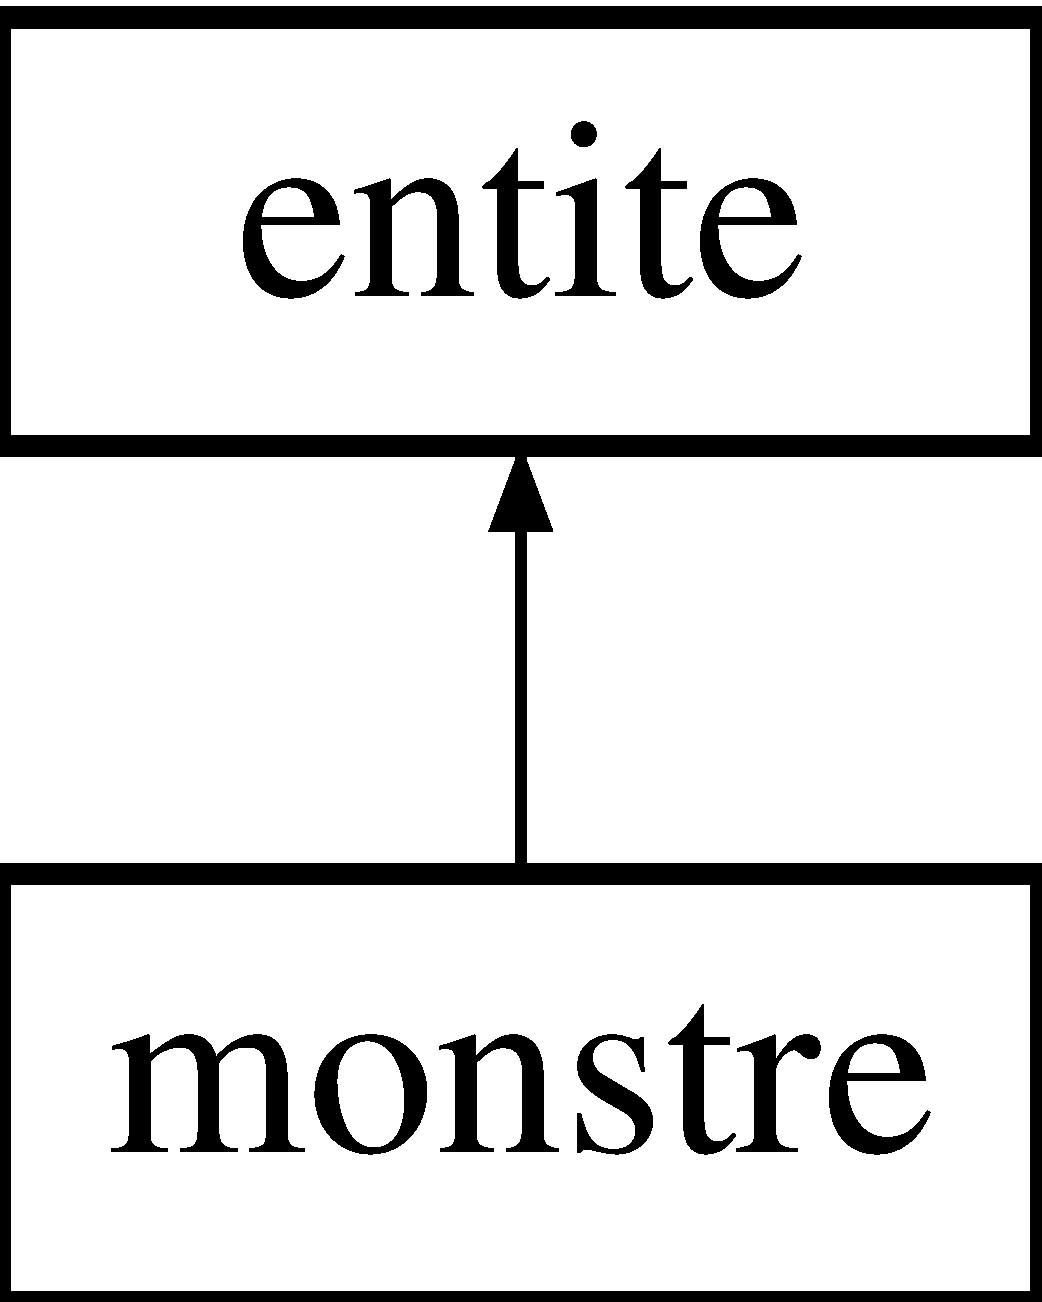
\includegraphics[height=2.000000cm]{classmonstre}
\end{center}
\end{figure}
\subsection*{Public Member Functions}
\begin{DoxyCompactItemize}
\item 
\hyperlink{classmonstre_a718cb1c5f9297f00e42e6b884ca85d6d}{monstre} ()
\begin{DoxyCompactList}\small\item\em Constructeur vide. \end{DoxyCompactList}\item 
\hyperlink{classmonstre_a863d9f9a553a2e3a49d16182dd004da8}{monstre} (std\+::string \hyperlink{classentite_a904e8783de9fe2fc4306bf6b7822d025}{entite\+Id}, std\+::string \hyperlink{classentite_abe631a515b1cd0866dcfb078c4ceb07a}{entite\+Name}, int \hyperlink{classentite_a754557f56c1c1fcbcbd40eec68b60f65}{entite\+Hp\+Max}, int \hyperlink{classentite_ad9df70a9bb07f07b3ebf520941c3a35f}{entite\+Speed}, int \hyperlink{classentite_a696167d32c27b3b2a2fa6b473a888b18}{entite\+Mana\+Max}, std\+::string \hyperlink{classentite_a6fab1d9a04ade2cb97ec0904b12c82c9}{entite\+Description}, std\+::vector$<$ \hyperlink{classcompetence}{competence} $>$ all\+Skills)
\begin{DoxyCompactList}\small\item\em Constructeur avec tout. \end{DoxyCompactList}\item 
void \hyperlink{classmonstre_aeb60395664bbca7846e037b058b5c716}{print\+Monstre} ()
\end{DoxyCompactItemize}
\subsection*{Static Public Attributes}
\begin{DoxyCompactItemize}
\item 
static int \hyperlink{classmonstre_a9de7f320e15973eca48ff44d7e94ae04}{nb\+Elem\+Prot}
\begin{DoxyCompactList}\small\item\em Nombre de monstres protégés. \end{DoxyCompactList}\end{DoxyCompactItemize}
\subsection*{Additional Inherited Members}


\subsection{Detailed Description}
Classe créant un monstre en mémoire. hérite des propriétés ainsi que des attributs de la classe entite. 

\subsection{Constructor \& Destructor Documentation}
\mbox{\Hypertarget{classmonstre_a718cb1c5f9297f00e42e6b884ca85d6d}\label{classmonstre_a718cb1c5f9297f00e42e6b884ca85d6d}} 
\index{monstre@{monstre}!monstre@{monstre}}
\index{monstre@{monstre}!monstre@{monstre}}
\subsubsection{\texorpdfstring{monstre()}{monstre()}\hspace{0.1cm}{\footnotesize\ttfamily [1/2]}}
{\footnotesize\ttfamily monstre\+::monstre (\begin{DoxyParamCaption}{ }\end{DoxyParamCaption})}



Constructeur vide. 

Crée un monstre vide. \begin{DoxyWarning}{Warning}
Le monstre sera vide. Cela signifie qu\textquotesingle{}il ne sera pas utilisable pour le jeu, sa vie étant égale à 0 
\end{DoxyWarning}
\begin{DoxyPostcond}{Postcondition}
Le monstre crée aura les paramètres suivants\+:
\begin{DoxyItemize}
\item entite\+Name = \char`\"{}\+Inconnu\char`\"{}
\item entite\+Hp\+Max = 0
\item entite\+Hp\+Current = 0
\item entite\+Speed = 0
\item entite\+Alive = true (sera changé immédiatement en false)
\item entite\+Skill\+Vect = $<$vecteur vide$>$=\char`\"{}\char`\"{}$>$ 
\end{DoxyItemize}
\end{DoxyPostcond}
\mbox{\Hypertarget{classmonstre_a863d9f9a553a2e3a49d16182dd004da8}\label{classmonstre_a863d9f9a553a2e3a49d16182dd004da8}} 
\index{monstre@{monstre}!monstre@{monstre}}
\index{monstre@{monstre}!monstre@{monstre}}
\subsubsection{\texorpdfstring{monstre()}{monstre()}\hspace{0.1cm}{\footnotesize\ttfamily [2/2]}}
{\footnotesize\ttfamily monstre\+::monstre (\begin{DoxyParamCaption}\item[{std\+::string}]{entite\+Id,  }\item[{std\+::string}]{entite\+Name,  }\item[{int}]{entite\+Hp\+Max,  }\item[{int}]{entite\+Speed,  }\item[{int}]{entite\+Mana\+Max,  }\item[{std\+::string}]{entite\+Description,  }\item[{std\+::vector$<$ \hyperlink{classcompetence}{competence} $>$}]{all\+Skills }\end{DoxyParamCaption})\hspace{0.3cm}{\ttfamily [inline]}}



Constructeur avec tout. 


\begin{DoxyParams}{Parameters}
{\em entite\+Id} & L\textquotesingle{}identifiant du monstre \\
\hline
{\em entite\+Name} & Le nom du monstre \\
\hline
{\em entite\+Hp\+Max} & Les points de vie max du monstre \\
\hline
{\em entite\+Speed} & La vitesse du monstre \\
\hline
{\em entite\+Mana\+Max} & Les points de mana max du monstre \\
\hline
{\em entite\+Description} & La description du monstre \\
\hline
{\em all\+Skills} & Un vecteur (std\+::vector) contenant toutes les compétences de ce monstre. \\
\hline
\end{DoxyParams}


\subsection{Member Function Documentation}
\mbox{\Hypertarget{classmonstre_aeb60395664bbca7846e037b058b5c716}\label{classmonstre_aeb60395664bbca7846e037b058b5c716}} 
\index{monstre@{monstre}!print\+Monstre@{print\+Monstre}}
\index{print\+Monstre@{print\+Monstre}!monstre@{monstre}}
\subsubsection{\texorpdfstring{print\+Monstre()}{printMonstre()}}
{\footnotesize\ttfamily void monstre\+::print\+Monstre (\begin{DoxyParamCaption}{ }\end{DoxyParamCaption})}



\subsection{Member Data Documentation}
\mbox{\Hypertarget{classmonstre_a9de7f320e15973eca48ff44d7e94ae04}\label{classmonstre_a9de7f320e15973eca48ff44d7e94ae04}} 
\index{monstre@{monstre}!nb\+Elem\+Prot@{nb\+Elem\+Prot}}
\index{nb\+Elem\+Prot@{nb\+Elem\+Prot}!monstre@{monstre}}
\subsubsection{\texorpdfstring{nb\+Elem\+Prot}{nbElemProt}}
{\footnotesize\ttfamily int monstre\+::nb\+Elem\+Prot\hspace{0.3cm}{\ttfamily [static]}}



Nombre de monstres protégés. 

Variable de classse permettant d\textquotesingle{}identifier le nombre de monstres par défaut ne pouvant pas être modifiés (sauf modification directe du code). 

The documentation for this class was generated from the following file\+:\begin{DoxyCompactItemize}
\item 
/\+Users/thibault/\+Git\+Hub/\+C\+E\+R\+I\+\_\+software\+\_\+engineering\+\_\+game\+\_\+1/headers/\hyperlink{monstre_8h}{monstre.\+h}\end{DoxyCompactItemize}

\hypertarget{classpersonnage}{}\section{personnage Class Reference}
\label{classpersonnage}\index{personnage@{personnage}}


{\ttfamily \#include $<$personnage.\+h$>$}

Inheritance diagram for personnage\+:\begin{figure}[H]
\begin{center}
\leavevmode
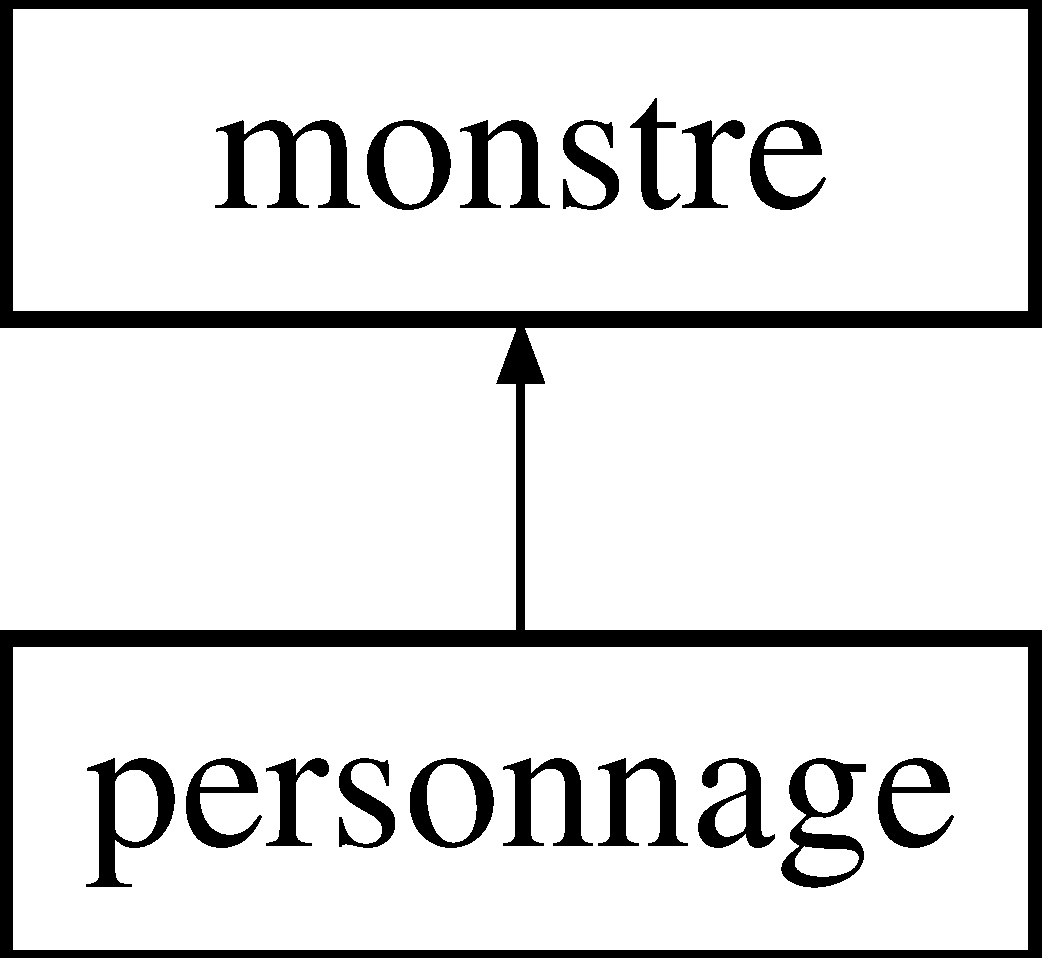
\includegraphics[height=2.000000cm]{classpersonnage}
\end{center}
\end{figure}
\subsection*{Public Member Functions}
\begin{DoxyCompactItemize}
\item 
\hyperlink{classpersonnage_acd9ca516f8c5c110687e5167dab8db59}{personnage} ()
\begin{DoxyCompactList}\small\item\em Constructeur vide. \end{DoxyCompactList}\item 
\hyperlink{classpersonnage_adec7b6f38637e7d176e054b68b0fcb23}{personnage} (std\+::string \hyperlink{classentite_a904e8783de9fe2fc4306bf6b7822d025}{entite\+Id}, std\+::string \hyperlink{classentite_abe631a515b1cd0866dcfb078c4ceb07a}{entite\+Name}, int \hyperlink{classentite_a754557f56c1c1fcbcbd40eec68b60f65}{entite\+Hp\+Max}, int \hyperlink{classentite_ad9df70a9bb07f07b3ebf520941c3a35f}{entite\+Speed}, int \hyperlink{classentite_a696167d32c27b3b2a2fa6b473a888b18}{entite\+Mana\+Max}, std\+::string \hyperlink{classentite_a6fab1d9a04ade2cb97ec0904b12c82c9}{entite\+Description}, std\+::vector$<$ \hyperlink{classcompetence}{competence} $>$ all\+Skills)
\item 
void \hyperlink{classpersonnage_a173f1b07d9098a96fd189ede2e7dad59}{print\+Personnage} ()
\begin{DoxyCompactList}\small\item\em Fonction de test. \end{DoxyCompactList}\end{DoxyCompactItemize}
\subsection*{Additional Inherited Members}


\subsection{Constructor \& Destructor Documentation}
\mbox{\Hypertarget{classpersonnage_acd9ca516f8c5c110687e5167dab8db59}\label{classpersonnage_acd9ca516f8c5c110687e5167dab8db59}} 
\index{personnage@{personnage}!personnage@{personnage}}
\index{personnage@{personnage}!personnage@{personnage}}
\subsubsection{\texorpdfstring{personnage()}{personnage()}\hspace{0.1cm}{\footnotesize\ttfamily [1/2]}}
{\footnotesize\ttfamily personnage\+::personnage (\begin{DoxyParamCaption}{ }\end{DoxyParamCaption})\hspace{0.3cm}{\ttfamily [inline]}}



Constructeur vide. 

Le personnage créé aura 0 de mana, et n\textquotesingle{}aura aucune description. Mais il sera crée. \mbox{\Hypertarget{classpersonnage_adec7b6f38637e7d176e054b68b0fcb23}\label{classpersonnage_adec7b6f38637e7d176e054b68b0fcb23}} 
\index{personnage@{personnage}!personnage@{personnage}}
\index{personnage@{personnage}!personnage@{personnage}}
\subsubsection{\texorpdfstring{personnage()}{personnage()}\hspace{0.1cm}{\footnotesize\ttfamily [2/2]}}
{\footnotesize\ttfamily personnage\+::personnage (\begin{DoxyParamCaption}\item[{std\+::string}]{entite\+Id,  }\item[{std\+::string}]{entite\+Name,  }\item[{int}]{entite\+Hp\+Max,  }\item[{int}]{entite\+Speed,  }\item[{int}]{entite\+Mana\+Max,  }\item[{std\+::string}]{entite\+Description,  }\item[{std\+::vector$<$ \hyperlink{classcompetence}{competence} $>$}]{all\+Skills }\end{DoxyParamCaption})\hspace{0.3cm}{\ttfamily [inline]}}



\subsection{Member Function Documentation}
\mbox{\Hypertarget{classpersonnage_a173f1b07d9098a96fd189ede2e7dad59}\label{classpersonnage_a173f1b07d9098a96fd189ede2e7dad59}} 
\index{personnage@{personnage}!print\+Personnage@{print\+Personnage}}
\index{print\+Personnage@{print\+Personnage}!personnage@{personnage}}
\subsubsection{\texorpdfstring{print\+Personnage()}{printPersonnage()}}
{\footnotesize\ttfamily void personnage\+::print\+Personnage (\begin{DoxyParamCaption}{ }\end{DoxyParamCaption})}



Fonction de test. 



The documentation for this class was generated from the following file\+:\begin{DoxyCompactItemize}
\item 
/\+Users/thibault/\+Git\+Hub/\+C\+E\+R\+I\+\_\+software\+\_\+engineering\+\_\+game\+\_\+1/headers/\hyperlink{personnage_8h}{personnage.\+h}\end{DoxyCompactItemize}

\chapter{File Documentation}
\hypertarget{carte_8h}{}\section{/\+Users/thibault/\+Git\+Hub/\+C\+E\+R\+I\+\_\+software\+\_\+engineering\+\_\+game\+\_\+1/headers/carte.h File Reference}
\label{carte_8h}\index{/\+Users/thibault/\+Git\+Hub/\+C\+E\+R\+I\+\_\+software\+\_\+engineering\+\_\+game\+\_\+1/headers/carte.\+h@{/\+Users/thibault/\+Git\+Hub/\+C\+E\+R\+I\+\_\+software\+\_\+engineering\+\_\+game\+\_\+1/headers/carte.\+h}}
{\ttfamily \#include $<$iostream$>$}\newline
{\ttfamily \#include $<$string$>$}\newline
{\ttfamily \#include $<$vector$>$}\newline
\subsection*{Classes}
\begin{DoxyCompactItemize}
\item 
class \hyperlink{class_carte}{Carte}
\begin{DoxyCompactList}\small\item\em Classe qui permet de modéliser une carte en mémoire. \end{DoxyCompactList}\end{DoxyCompactItemize}

\hypertarget{competence_8h}{}\section{/\+Users/thibault/\+Git\+Hub/\+C\+E\+R\+I\+\_\+software\+\_\+engineering\+\_\+game\+\_\+1/headers/competence.h File Reference}
\label{competence_8h}\index{/\+Users/thibault/\+Git\+Hub/\+C\+E\+R\+I\+\_\+software\+\_\+engineering\+\_\+game\+\_\+1/headers/competence.\+h@{/\+Users/thibault/\+Git\+Hub/\+C\+E\+R\+I\+\_\+software\+\_\+engineering\+\_\+game\+\_\+1/headers/competence.\+h}}
{\ttfamily \#include $<$iostream$>$}\newline
{\ttfamily \#include $<$sstream$>$}\newline
{\ttfamily \#include $<$string$>$}\newline
\subsection*{Classes}
\begin{DoxyCompactItemize}
\item 
class \hyperlink{classcompetence}{competence}
\end{DoxyCompactItemize}

\hypertarget{entite_8h}{}\section{/\+Users/thibault/\+Git\+Hub/\+C\+E\+R\+I\+\_\+software\+\_\+engineering\+\_\+game\+\_\+1/headers/entite.h File Reference}
\label{entite_8h}\index{/\+Users/thibault/\+Git\+Hub/\+C\+E\+R\+I\+\_\+software\+\_\+engineering\+\_\+game\+\_\+1/headers/entite.\+h@{/\+Users/thibault/\+Git\+Hub/\+C\+E\+R\+I\+\_\+software\+\_\+engineering\+\_\+game\+\_\+1/headers/entite.\+h}}
{\ttfamily \#include $<$string$>$}\newline
{\ttfamily \#include $<$vector$>$}\newline
{\ttfamily \#include \char`\"{}competence.\+h\char`\"{}}\newline
\subsection*{Classes}
\begin{DoxyCompactItemize}
\item 
class \hyperlink{classentite}{entite}
\end{DoxyCompactItemize}

\hypertarget{fonctionsjeu_8h}{}\section{/\+Users/thibault/\+Git\+Hub/\+C\+E\+R\+I\+\_\+software\+\_\+engineering\+\_\+game\+\_\+1/headers/fonctionsjeu.h File Reference}
\label{fonctionsjeu_8h}\index{/\+Users/thibault/\+Git\+Hub/\+C\+E\+R\+I\+\_\+software\+\_\+engineering\+\_\+game\+\_\+1/headers/fonctionsjeu.\+h@{/\+Users/thibault/\+Git\+Hub/\+C\+E\+R\+I\+\_\+software\+\_\+engineering\+\_\+game\+\_\+1/headers/fonctionsjeu.\+h}}
{\ttfamily \#include $<$stack$>$}\newline
{\ttfamily \#include $<$vector$>$}\newline
{\ttfamily \#include \char`\"{}../headers/carte.\+h\char`\"{}}\newline
{\ttfamily \#include \char`\"{}../headers/competence.\+h\char`\"{}}\newline
{\ttfamily \#include \char`\"{}../headers/io.\+h\char`\"{}}\newline
{\ttfamily \#include \char`\"{}../headers/monstre.\+h\char`\"{}}\newline
{\ttfamily \#include \char`\"{}../headers/personnage.\+h\char`\"{}}\newline
\subsection*{Classes}
\begin{DoxyCompactItemize}
\item 
class \hyperlink{classjeu}{jeu}
\begin{DoxyCompactList}\small\item\em Ceci sera la classe du jeu. Elle contient toutes les entités, la carte, ainsi que les fonctions nécessaires à la partie. \end{DoxyCompactList}\end{DoxyCompactItemize}
\subsection*{Functions}
\begin{DoxyCompactItemize}
\item 
bool \hyperlink{fonctionsjeu_8h_a50b5865580161a893e2e90d8dff249db}{sort\+\_\+speed} (\hyperlink{classentite}{entite} a, \hyperlink{classentite}{entite} b)
\begin{DoxyCompactList}\small\item\em Tri d\textquotesingle{}entités. \end{DoxyCompactList}\end{DoxyCompactItemize}


\subsection{Function Documentation}
\mbox{\Hypertarget{fonctionsjeu_8h_a50b5865580161a893e2e90d8dff249db}\label{fonctionsjeu_8h_a50b5865580161a893e2e90d8dff249db}} 
\index{fonctionsjeu.\+h@{fonctionsjeu.\+h}!sort\+\_\+speed@{sort\+\_\+speed}}
\index{sort\+\_\+speed@{sort\+\_\+speed}!fonctionsjeu.\+h@{fonctionsjeu.\+h}}
\subsubsection{\texorpdfstring{sort\+\_\+speed()}{sort\_speed()}}
{\footnotesize\ttfamily bool sort\+\_\+speed (\begin{DoxyParamCaption}\item[{\hyperlink{classentite}{entite}}]{a,  }\item[{\hyperlink{classentite}{entite}}]{b }\end{DoxyParamCaption})}



Tri d\textquotesingle{}entités. 

Trie des entités selon la valeur de leur attribut de vitesse. 
\begin{DoxyParams}{Parameters}
{\em a} & Entité par rapport à laquelle on trie. \\
\hline
{\em b} & Entité à trier. \\
\hline
\end{DoxyParams}
\begin{DoxyReturn}{Returns}
Un booléen\+: true si la vitesse de a est supérieure à la vitesse de b. 
\end{DoxyReturn}

\hypertarget{io_8h}{}\section{/\+Users/thibault/\+Git\+Hub/\+C\+E\+R\+I\+\_\+software\+\_\+engineering\+\_\+game\+\_\+1/headers/io.h File Reference}
\label{io_8h}\index{/\+Users/thibault/\+Git\+Hub/\+C\+E\+R\+I\+\_\+software\+\_\+engineering\+\_\+game\+\_\+1/headers/io.\+h@{/\+Users/thibault/\+Git\+Hub/\+C\+E\+R\+I\+\_\+software\+\_\+engineering\+\_\+game\+\_\+1/headers/io.\+h}}
{\ttfamily \#include $<$algorithm$>$}\newline
{\ttfamily \#include $<$fstream$>$}\newline
{\ttfamily \#include $<$iostream$>$}\newline
{\ttfamily \#include $<$sstream$>$}\newline
{\ttfamily \#include $<$stdio.\+h$>$}\newline
{\ttfamily \#include $<$termios.\+h$>$}\newline
{\ttfamily \#include $<$typeinfo$>$}\newline
{\ttfamily \#include $<$vector$>$}\newline
{\ttfamily \#include \char`\"{}../headers/carte.\+h\char`\"{}}\newline
{\ttfamily \#include \char`\"{}../headers/competence.\+h\char`\"{}}\newline
{\ttfamily \#include \char`\"{}../headers/entite.\+h\char`\"{}}\newline
{\ttfamily \#include \char`\"{}../headers/monstre.\+h\char`\"{}}\newline
{\ttfamily \#include \char`\"{}../headers/personnage.\+h\char`\"{}}\newline
\subsection*{Namespaces}
\begin{DoxyCompactItemize}
\item 
 \hyperlink{namespaceio}{io}
\begin{DoxyCompactList}\small\item\em Cet espace sera un espace permettant de définir un buffer custom pour les input, ainsi que de pouvoir afficher tout ce que l\textquotesingle{}on souhaite. \end{DoxyCompactList}\end{DoxyCompactItemize}
\subsection*{Macros}
\begin{DoxyCompactItemize}
\item 
\#define \hyperlink{io_8h_a7a88fe5b19b9d27c4d2b2d2501f8591a}{I\+O\+\_\+H}
\end{DoxyCompactItemize}
\subsection*{Functions}
\begin{DoxyCompactItemize}
\item 
void \hyperlink{namespaceio_ac0223d0ecfee82d8cc86543604173b73}{io\+::\+Change\+Terminal} (bool Ech=0)
\begin{DoxyCompactList}\small\item\em Changement des paramètres du terminal. \end{DoxyCompactList}\item 
void \hyperlink{namespaceio_a44a79937063c75bdcd8f042d5f55d501}{io\+::\+Reset\+Terminal} ()
\begin{DoxyCompactList}\small\item\em Remet le terminal à zero. \end{DoxyCompactList}\item 
int \hyperlink{namespaceio_a71636a15a219ee1dcc177e9749cf20bc}{io\+::get\+Terminal\+Width} ()
\begin{DoxyCompactList}\small\item\em Retourne la largeur du terminal. \end{DoxyCompactList}\item 
int \hyperlink{namespaceio_ab7da8a98a7b636d1d5f0f6eb820f1f81}{io\+::get\+Terminal\+Height} ()
\begin{DoxyCompactList}\small\item\em Retourne la hauteur du terminal. \end{DoxyCompactList}\item 
void \hyperlink{namespaceio_abefd9b2fada48d5e8e260e56e868e952}{io\+::clear\+Screen} ()
\begin{DoxyCompactList}\small\item\em Efface l\textquotesingle{}écran. \end{DoxyCompactList}\item 
void \hyperlink{namespaceio_a5a0d785914a680440e4986a02b50a28e}{io\+::check\+Terminal\+Size} ()
\begin{DoxyCompactList}\small\item\em Vérifie la taille du terminal. \end{DoxyCompactList}\item 
char \hyperlink{namespaceio_ae9908b55f26f07e78043d7cfad003d22}{io\+::de} ()
\begin{DoxyCompactList}\small\item\em Input. \end{DoxyCompactList}\item 
std\+::string \hyperlink{namespaceio_ab044be3afd7ac04eeb1a496af0f1d5c6}{io\+::long\+\_\+input} ()
\begin{DoxyCompactList}\small\item\em Entrée utilisateur contenant plus d\textquotesingle{}un caractère. \end{DoxyCompactList}\item 
void \hyperlink{namespaceio_ad1c0f5f45e4ec19ee5dbc108314eacbc}{io\+::afficher\+Carte} (\hyperlink{class_carte}{Carte} \&, int, bool reset=1)
\begin{DoxyCompactList}\small\item\em Affichage de la carte. \end{DoxyCompactList}\item 
void \hyperlink{namespaceio_ae9438bfe8b2631be82b0f4d644358545}{io\+::update\+Map} (\hyperlink{class_carte}{Carte} \&jeu\+\_\+carte, std\+::pair$<$ int, int $>$ new\+Player\+Pos)
\begin{DoxyCompactList}\small\item\em Met à jour l\textquotesingle{}affichage de la carte. \end{DoxyCompactList}\item 
void \hyperlink{namespaceio_a7fdf85a0d766d2dcdb9870ae0458826a}{io\+::bienvenue} ()
\begin{DoxyCompactList}\small\item\em Message d\textquotesingle{}accueil. \end{DoxyCompactList}\item 
void \hyperlink{namespaceio_ac60b7c3503eb53e69a2adc86368ab633}{io\+::afficher\+Mouvements} ()
\begin{DoxyCompactList}\small\item\em Fonction permettant d\textquotesingle{}afficher un overlay sur la carte. \end{DoxyCompactList}\item 
void \hyperlink{namespaceio_a45e9ac702aa6ea62eeca96e921b8eaa1}{io\+::afficher\+Mouvements} (std\+::string erreur\+\_\+deplacement)
\begin{DoxyCompactList}\small\item\em Fonction permettant d\textquotesingle{}afficher un overlay sur la carte. \end{DoxyCompactList}\item 
void \hyperlink{namespaceio_ac0728fb89b032a7b33641e0d2c34cc28}{io\+::afficher\+Mouvements} (std\+::string deplacements\+\_\+possibles, std\+::string erreur\+\_\+deplacement)
\begin{DoxyCompactList}\small\item\em Fonction permettant d\textquotesingle{}afficher un overlay sur la carte. \end{DoxyCompactList}\item 
void \hyperlink{namespaceio_a312765b285c5f20dfe113609c86b8fdd}{io\+::afficher\+Mouvements} (std\+::string message, std\+::string deplacements\+\_\+possibles, std\+::string erreur\+\_\+deplacement)
\begin{DoxyCompactList}\small\item\em Fonction permettant d\textquotesingle{}afficher un overlay sur la carte. \end{DoxyCompactList}\item 
void \hyperlink{namespaceio_a61739b6fe40275cdb72215fd08f41d87}{io\+::update\+Message} (std\+::string s, int pos)
\item 
void \hyperlink{namespaceio_a0ed486192687092d372440a79c3a65a3}{io\+::remove\+Last\+Char} (std\+::stringstream \&i)
\begin{DoxyCompactList}\small\item\em Enlève le dernier caractère d\textquotesingle{}un stringstream. \end{DoxyCompactList}\item 
bool \hyperlink{namespaceio_ac79ddb3191a9d00d007eb48deb315942}{io\+::check\+Input} (int x)
\begin{DoxyCompactList}\small\item\em Vérifie que l\textquotesingle{}user entre des entiers. \end{DoxyCompactList}\item 
bool \hyperlink{namespaceio_a993e82931eec7bf1db5110871c03c2d1}{io\+::check\+Separator\+Entite} (std\+::string une\+Ligne)
\begin{DoxyCompactList}\small\item\em Verifie qu\textquotesingle{}une ligne est correcte dans un fichier texte d\textquotesingle{}entités (bon nombre de séparateurs) + //! Créer une competence. \end{DoxyCompactList}\item 
bool \hyperlink{namespaceio_ae543bba7ec112a88734317ca61bbb88a}{io\+::check\+Separator\+Skill} (std\+::string nom\+Fichier, int num\+Ligne)
\begin{DoxyCompactList}\small\item\em Verifie qu\textquotesingle{}un champ compétences est correct dans un fichier texte d\textquotesingle{}entités (bon nombre de séparateurs) \end{DoxyCompactList}\item 
int \hyperlink{namespaceio_a0161a5c00ad8e7222f3a052e7c9fa67b}{io\+::taille\+\_\+str} (std\+::string)
\begin{DoxyCompactList}\small\item\em Compte la taille d\textquotesingle{}une string mieux que la fonction std\+::string\+::size(), car elle ne compte pas les accents comme deux caractères. \end{DoxyCompactList}\item 
void \hyperlink{namespaceio_ac1340cd13ac838a1d1cfaa0d25a4bbfb}{io\+::set\+Player\+Position} (int, int)
\item 
int \hyperlink{namespaceio_a495fffe3be2fea58511cedcfcea5dbbd}{io\+::\+To\+\_\+int} (std\+::string input)
\begin{DoxyCompactList}\small\item\em Convertit un string en int. \end{DoxyCompactList}\item 
{\footnotesize template$<$typename T $>$ }\\void \hyperlink{namespaceio_ac5222293c3d12f7982a8df7ead04ba0b}{io\+::afficher} (T object)
\begin{DoxyCompactList}\small\item\em Affichage d\textquotesingle{}objet. \end{DoxyCompactList}\item 
{\footnotesize template$<$typename T $>$ }\\void \hyperlink{namespaceio_acf5693654c155fd094993bf20ac39343}{io\+::liste\+\_\+elements} (std\+::vector$<$ T $>$ vect\+\_\+element)
\begin{DoxyCompactList}\small\item\em Affichage d\textquotesingle{}un ensemble d\textquotesingle{}objets. \end{DoxyCompactList}\item 
{\footnotesize template$<$typename T $>$ }\\void \hyperlink{namespaceio_ad045ca63d3481c2da3253a3944df18e4}{io\+::choix\+\_\+unique\+\_\+element} (T \&element, std\+::vector$<$ T $>$ vect\+\_\+element, bool combat, bool aff=1)
\begin{DoxyCompactList}\small\item\em Choix d\textquotesingle{}un élément unique. \end{DoxyCompactList}\item 
void \hyperlink{namespaceio_aea8dfd5fea1f29722c77b31ef7b0b940}{io\+::aff\+\_\+combat} (std\+::vector$<$ \hyperlink{classentite}{entite} $>$ vect\+\_\+entite)
\begin{DoxyCompactList}\small\item\em Affichage des entités du combat. \end{DoxyCompactList}\item 
std\+::vector$<$ \hyperlink{classcompetence}{competence} $>$ \hyperlink{namespaceio_a9297653474b9ce9930d6a3862401e751}{io\+::load\+Competence\+From\+File} (std\+::string nom\+Fichier, int num\+Ligne)
\begin{DoxyCompactList}\small\item\em Chargement des compétences. \end{DoxyCompactList}\item 
std\+::vector$<$ \hyperlink{class_carte}{Carte} $>$ \hyperlink{namespaceio_abb49308ca24862cc2b64c8c15949af44}{io\+::load\+All\+Carte\+From\+File} (std\+::string nom\+Fichier)
\begin{DoxyCompactList}\small\item\em Chargement des cartes. \end{DoxyCompactList}\item 
{\footnotesize template$<$typename T $>$ }\\std\+::vector$<$ T $>$ \hyperlink{namespaceio_a97ddce5128c7df7d67966208e2c37c4c}{io\+::load\+All\+Entite\+From\+File} (T temp, std\+::string nom\+Fichier)
\begin{DoxyCompactList}\small\item\em Chargement des entités. \end{DoxyCompactList}\item 
{\footnotesize template$<$typename T $>$ }\\std\+::string \hyperlink{namespaceio_adfc4ec23f63d0f743773a584f0a5826f}{io\+::to\+String} (const T \&valeur)
\item 
bool \hyperlink{namespaceio_ad825d53d81ddd635e3875dfb9d54f627}{io\+::input\+Sep\+Check} (std\+::string input)
\end{DoxyCompactItemize}
\subsection*{Variables}
\begin{DoxyCompactItemize}
\item 
int \hyperlink{namespaceio_a09b19ec88fb58a6086ca54be52b7bc08}{io\+::\+Term\+Width}
\begin{DoxyCompactList}\small\item\em Variable retennant la valeur de la largeur de la fenêtre du terminal. Elle permet de réduire le nombre de calculs à faire (étant donné que cette valeur est obtenue avec l\textquotesingle{}ouverture d\textquotesingle{}un fichier, son calcul prends donc quelques temps). \end{DoxyCompactList}\item 
int \hyperlink{namespaceio_afaeef00a45e14dc7227025fa7fd27240}{io\+::\+Term\+Height}
\begin{DoxyCompactList}\small\item\em Variable retennant la valeur de la hauteur de la fenêtre du terminal. Elle permet de réduire le nombre de calculs à faire (étant donné que cette valeur est obtenue avec l\textquotesingle{}ouverture d\textquotesingle{}un fichier, son calcul prends donc quelques temps). \end{DoxyCompactList}\item 
std\+::string \hyperlink{namespaceio_a24918bdd47093eb3f11b694ad6f832d4}{io\+::\+B\+L\+A\+NK}
\begin{DoxyCompactList}\small\item\em Chaîne de caractères permettant de remettre à zéro la couleur du texte. \end{DoxyCompactList}\item 
std\+::string \hyperlink{namespaceio_ac9181eea4e6d57e5481bc7e5822de4cb}{io\+::\+R\+ED}
\begin{DoxyCompactList}\small\item\em Chaîne de caractères permettant de rendre le texte affiché de couleur rouge. \end{DoxyCompactList}\item 
std\+::string \hyperlink{namespaceio_a38fffa22831731f5fc0b72700dc75c87}{io\+::\+G\+R\+E\+EN}
\begin{DoxyCompactList}\small\item\em Chaîne de caractères permettant de rendre le texte affiché de couleur verte. \end{DoxyCompactList}\item 
std\+::string \hyperlink{namespaceio_a0bb7c89e9e48840601811e4e35421767}{io\+::\+Y\+E\+L\+L\+OW}
\begin{DoxyCompactList}\small\item\em Chaîne de caractères permettant de rendre le texte affiché de couleur jaune. \end{DoxyCompactList}\item 
std\+::string \hyperlink{namespaceio_aad76ed62886e76ca53a755d1c917e387}{io\+::\+B\+L\+UE}
\begin{DoxyCompactList}\small\item\em Chaîne de caractères permettant de rendre le texte affiché de couleur bleue. \end{DoxyCompactList}\item 
std\+::string \hyperlink{namespaceio_a1e4a43cea85f576e62aebce6aabc60b5}{io\+::\+M\+A\+G\+E\+N\+TA}
\begin{DoxyCompactList}\small\item\em Chaîne de caractères permettant de rendre le texte affiché de couleur magenta. \end{DoxyCompactList}\item 
int \hyperlink{namespaceio_a7f2af984af03881a45da957db2c48be2}{io\+::map\+PositionX}
\begin{DoxyCompactList}\small\item\em Variable permettant de retenir à partir de quelle coordonnée \char`\"{}x\char`\"{} la carte est affichée (si la carte est plus grande que la fenêtre de terminal, cette valeur ne sera pas toujours à 0 ...) \end{DoxyCompactList}\item 
int \hyperlink{namespaceio_aa0322ffa705df7bd3c4fa5eaefde5d6d}{io\+::map\+Positiony}
\begin{DoxyCompactList}\small\item\em Variable permettant de retenir à partir de quelle coordonnée \char`\"{}y\char`\"{} la carte est affichée (si la carte est plus grande que la fenêtre de terminal, cette valeur ne sera pas toujours à 0 ...) \end{DoxyCompactList}\item 
int \hyperlink{namespaceio_af6147c2896f77caaa4c7d26daee44ac5}{io\+::interactions\+OverlayY}
\begin{DoxyCompactList}\small\item\em Stocke la position (x) de l\textquotesingle{}affichage de l\textquotesingle{}overlay des actions. Nous n\textquotesingle{}avons pas besoin du Y car l\textquotesingle{}overlay prends toute la largeur quoi qu\textquotesingle{}il arrive. \end{DoxyCompactList}\item 
std\+::pair$<$ int, int $>$ \hyperlink{namespaceio_a2a0c75ff7760b96fcf6e696efe3d1c51}{io\+::current\+Player\+Position}
\begin{DoxyCompactList}\small\item\em Paire de valeurs (std\+::pair) gardant la position actuelle du joueur dans. \end{DoxyCompactList}\end{DoxyCompactItemize}


\subsection{Macro Definition Documentation}
\mbox{\Hypertarget{io_8h_a7a88fe5b19b9d27c4d2b2d2501f8591a}\label{io_8h_a7a88fe5b19b9d27c4d2b2d2501f8591a}} 
\index{io.\+h@{io.\+h}!I\+O\+\_\+H@{I\+O\+\_\+H}}
\index{I\+O\+\_\+H@{I\+O\+\_\+H}!io.\+h@{io.\+h}}
\subsubsection{\texorpdfstring{I\+O\+\_\+H}{IO\_H}}
{\footnotesize\ttfamily \#define I\+O\+\_\+H}


\hypertarget{monstre_8h}{}\section{/\+Users/thibault/\+Git\+Hub/\+C\+E\+R\+I\+\_\+software\+\_\+engineering\+\_\+game\+\_\+1/headers/monstre.h File Reference}
\label{monstre_8h}\index{/\+Users/thibault/\+Git\+Hub/\+C\+E\+R\+I\+\_\+software\+\_\+engineering\+\_\+game\+\_\+1/headers/monstre.\+h@{/\+Users/thibault/\+Git\+Hub/\+C\+E\+R\+I\+\_\+software\+\_\+engineering\+\_\+game\+\_\+1/headers/monstre.\+h}}
{\ttfamily \#include \char`\"{}../headers/entite.\+h\char`\"{}}\newline
\subsection*{Classes}
\begin{DoxyCompactItemize}
\item 
class \hyperlink{classmonstre}{monstre}
\begin{DoxyCompactList}\small\item\em Classe créant un monstre en mémoire. hérite des propriétés ainsi que des attributs de la classe entite. \end{DoxyCompactList}\end{DoxyCompactItemize}

\hypertarget{personnage_8h}{}\section{/\+Users/thibault/\+Git\+Hub/\+C\+E\+R\+I\+\_\+software\+\_\+engineering\+\_\+game\+\_\+1/headers/personnage.h File Reference}
\label{personnage_8h}\index{/\+Users/thibault/\+Git\+Hub/\+C\+E\+R\+I\+\_\+software\+\_\+engineering\+\_\+game\+\_\+1/headers/personnage.\+h@{/\+Users/thibault/\+Git\+Hub/\+C\+E\+R\+I\+\_\+software\+\_\+engineering\+\_\+game\+\_\+1/headers/personnage.\+h}}
{\ttfamily \#include \char`\"{}../headers/entite.\+h\char`\"{}}\newline
\subsection*{Classes}
\begin{DoxyCompactItemize}
\item 
class \hyperlink{classpersonnage}{personnage}
\begin{DoxyCompactList}\small\item\em Classe personnage héritant de la classe entité \end{DoxyCompactList}\end{DoxyCompactItemize}

%--- End generated contents ---

% Index
\backmatter
\newpage
\phantomsection
\clearemptydoublepage
\addcontentsline{toc}{chapter}{Index}
\printindex

\end{document}
